\chapter{\ifproject%
\ifcpe โครงสร้างและขั้นตอนการทำงาน\else Project Structure and Methodology\fi
\else%
\ifcpe โครงสร้างของโครงงาน\else Project Structure\fi
\fi
}



\makeatletter

% \renewcommand\section{\@startsection {section}{1}{\z@}%
%                                    {13.5ex \@plus -1ex \@minus -.2ex}%
%                                    {2.3ex \@plus.2ex}%
%                                    {\normalfont\large\bfseries}}

\makeatother
%\vspace{2ex}
% \titleformat{\section}{\normalfont\bfseries}{\thesection}{1em}{}
% \titlespacing*{\section}{0pt}{10ex}{0pt}



\section{โครงสร้างของระบบ}



\subsection{Database Design}

ประเภทของฐานข้อมูลที่ใช้เป็นแบบ NoSQL
(รูปที่~\ref{fig:DatabaseDiagram}) แสดงองค์ประกอบต่างๆของฐานข้อมูล ซึ่งมีรายละเอียดดังต่อไปนี้
%
  \begin{itemize}
    \item childs เก็บข้อมูลที่เกี่ยวข้องกับเด็กทั้งหมด เช่น เก็บวันที่สมัคร วันที่เข้าเรียน ชื่อ ชื่อเล่น วันเดือนปีเกิด เป็นต้น  
    โดยที่ \_id จะมีการเชื่อมกับ payment, gadgets, healths, enrollment, address, guardians, customer, childStatic, childDynamic, medical, document, child\_info 
    ในส่วนของการเชื่อมความสัมพันธ์นี้ ทำเพื่อให้เวลาจะมีการเรียกใช้ข้อมูลของเด็กใน ส่วนของข้อมูลอื่น เช่น การเช็คชื่อ การชำระเงินค่าเรียน การเช็คของ การทำเช่นนี้จะช่วยให้เรียกข้อมูลเด็กมาใช้ได้ง่ายยิ่งขึ้น
    \item childStatic เก็บข้อมูลเด็กที่ไม่เปลี่ยนแปลง เชื้อชาติ ศาสนา วันที่สมัคร
    \item childDynamic เก็บข้อมูลเด็กที่มีการเปลี่ยนแปลง น้ำหนัก ส่วนสูง รูปถ่าย
    \item child\_info เก็บข้อมูลพฤติกรรมต่างๆของเด็ก
    \item info\_category เก็บข้อมูลชื่อประเภทหัวเรื่องต่างๆ
    \item info\_item เก็บข้อมูลหยิบย่อยต่างๆ
    \item info\_display\_order เก็บข้อมูลสำหรับทำหน้าแสดงผลแบบ dynamic
    \item customer เก็บข้อมูลลูกค้าสำหรับใช้ซื้อของจากทางเนอสเซอรี่
    \item medical เก็บข้อมูลทางการแพทย์ของเด็ก
    \item document เก็บข้อมูลเอกสารในการสมัครของเด็ก
    \item guardians เก็บข้อมูลส่วนตัวของผู้ปกครองเด็ก เช่น ชื่อ ทำอาชีพอะไร อีเมล เบอร์โทร มีความสัมพันธ์อะไรกับเด็ก เป็นต้น
    \item address เก็บข้อมูลที่อยู่ของเด็ก เช่น บ้านเลขที่ ถนน ตำบล อำเภอ จังหวัด รหัสไปรษณีย์ 
    \item users เก็บ email password สำหรับเข้าสู่ ระบบจัดการ nursery 
    \item rooms เก็บข้อมูลห้องเรียนว่าห้องนี้ชื่อห้องว่าอะไร ไว้ให้ enrollment เรียกใช้ผ่าน ObjectId
    \item enrollment เก็บข้อมูลว่าเด็กเริ่มเรียนห้องนี้วันไหน มีการย้ายออกจากห้องนี้วันไหน
    \item attendances เก็บข้อมูลการเช็คชื่อทั้งหมด วันที่เช็ค สถานะว่ามาหรือไม่มา
    \item gadgets เก็บข้อมูลการเช็คอุปกรณ์ของเด็กทั้งหมด มีการเก็บ ข้อมูลเด็ก วัน ลิสต์ของที่ต้องเช็ค ก็จะมีสถานะว่าเอามาหรือไม่เอามา
    \item healths เก็บข้อมูลการเช็คสุขภาพของเด็กทั้งหมด มีการเก็บ ข้อมูลเด็ก วัน ลิสต์สุขภาพที่ต้องเช็ค ก็จะมีสถานะว่าใช่หรือไม่ใช่
    \item stock เก็บข้อมูลของใช้ทั้งหมดของเด็กใน nursery ว่าของชิ้นนี้ชื่ออะไร ไซต์อะไร รหัสสินค้าคืออะไร
    \item show\_stock เก็บข้อมูลว่าของต่างๆมีจำนวนเท่าไหร่ ราคาเท่าไหร่
    \item history\_stock เก็บข้อมูลการเพิ่มลดของต่างๆ จำนวน แก้ไขวันไหน โดยใคร
    \item payment เก็บข้อมูลประวัติการโอนเงินค่าเล่าเรียนของผู้ปกครองเด็ก มีการเก็บ ข้อมูลเด็ก วันที่ส่งสลิปโอนเงิน ค่าเล่าเรียนหรือจำนวนเงินที่ชำระ รูปสลิปใบเสร็จ 
  \end{itemize}

\subsection{XD Design}

\begin{enumerate}
  \item RegisterPage คือ หน้าแบบฟอร์มในการลงทะเบียนเด็กในการเข้าเรียน nursery (รูปที่~\ref{fig:register}, \ref{fig:docForm})
  \item  ProfilePage คือ หน้าที่ใช้ในการจัดการกับประวัติส่วนตัวของเด็ก สามารถแสดงข้อมูลและแก้ไขข้อมูลของเด็กแต่ละคนได้ (รูปที่~\ref{fig:Profile}, \ref{fig:ChartPage}, \ref{fig:ProfileTwo}, \ref{fig:UpdateProfile})
  \item  Attendance คือ หน้าเช็คชื่อเด็กรายวัน (รูปที่~\ref{fig:Attendance}, \ref{fig:CheckAttendance})
  \item  Health คือ หน้าเช็คสุขภาพเด็กรายวัน (รูปที่~\ref{fig:Health}, \ref{fig:CheckHealth}) 
  \item  Gadget คือ หน้าเช็คของเด็กรายวัน (รูปที่~\ref{fig:Gadget}, \ref{fig:CheckGadget}) 
  \item  Stock คือ หน้าจัดการของใช้สำหรับเด็กทั้งหมดใน nursery (รูปที่~\ref{fig:Stock}, \ref{fig:CheckStock}, \ref{fig:editPrice}, \ref{fig:HistoryStock}) 
  \item  Payment คือ หน้าที่ใช้จัดการกับใบเสร็จ ประวัติการจ่ายเงินค่าเล่าเรียน (รูปที่~\ref{fig:Payment}, \ref{fig:CreatePayment}, \ref{fig:updatePayment}, \ref{fig:invoicePage}, \ref{fig:slipPage}) 
\end{enumerate}

\subsection{Architecture}

ระบบหลักๆที่ทางผู้พัฒนาใช้เป็นระบบแบบ Client-Server คือทางฝั่ง client จะใช้ React ในการพัฒนาตัวเว็บไซต์ โดยผู้ใช้จะมีการส่ง request มายังฝั่ง server เพื่อที่จะทำงานที่ผู้ใช้ต้องการ ซึ่งฝั่ง server 
จะพัฒนาผ่าน Express.js ทางฝั่งนี้ก็จะ query ข้อมูลจากทางฐานข้อมูลที่เก็บไว้บน MongoDB Atlas เมื่อได้รับข้อมูลแล้วจะทำการส่ง response กลับไปยัง client เพื่อให้ผู้ใช้สามารถทำงานในส่วนที่ต้องการได้

\subsection{APIs Docs}
(รูปที่~\ref{fig:ApiDocs1}, \ref{fig:ApiDocs2})
\section{ขั้นตอนการดำเนินงาน}
\subsection{Discovery}
\begin{itemize}
  \item สำรวจและสอบถามปัญหาจาก stakeholder
  \item นำปัญหาต่างหรือ requirements มาวิเคราะห์
  \item สรุปผลแล้วนำ requirements ที่ได้จากการวิเคราะห์ไปทำต่อในขั้นตอนถัดไป
\end{itemize}

\subsection{Design}
\begin{itemize}
  \item ออกแบบหน้า UI/UX โดย Adobe XD
  \item ออกแบบฐานข้อมูลโดย Draw.io
\end{itemize}

\subsection{Develop}
\begin{itemize}
  \item สร้าง Database
  \item เขียน APIs ตามที่ได้ design มาในขั้นตอนก่อนหน้า
  \item เขียน Frontend แล้วทดสอบยิง APIs ไปยังฝั่ง Backend
  \item เชื่อมโค้ด Frontend กับ Backend ผ่าน APIs
\end{itemize}

\subsection{Testing}
\begin{itemize}
  \item ทดสอบระบบในแต่ละฟีเจอร์ว่าสามารถใช้งานได้ตามที่ต้องการหรือไม่
\end{itemize}

\begin{landscape}
  \begin{figure}
    \begin{center}
    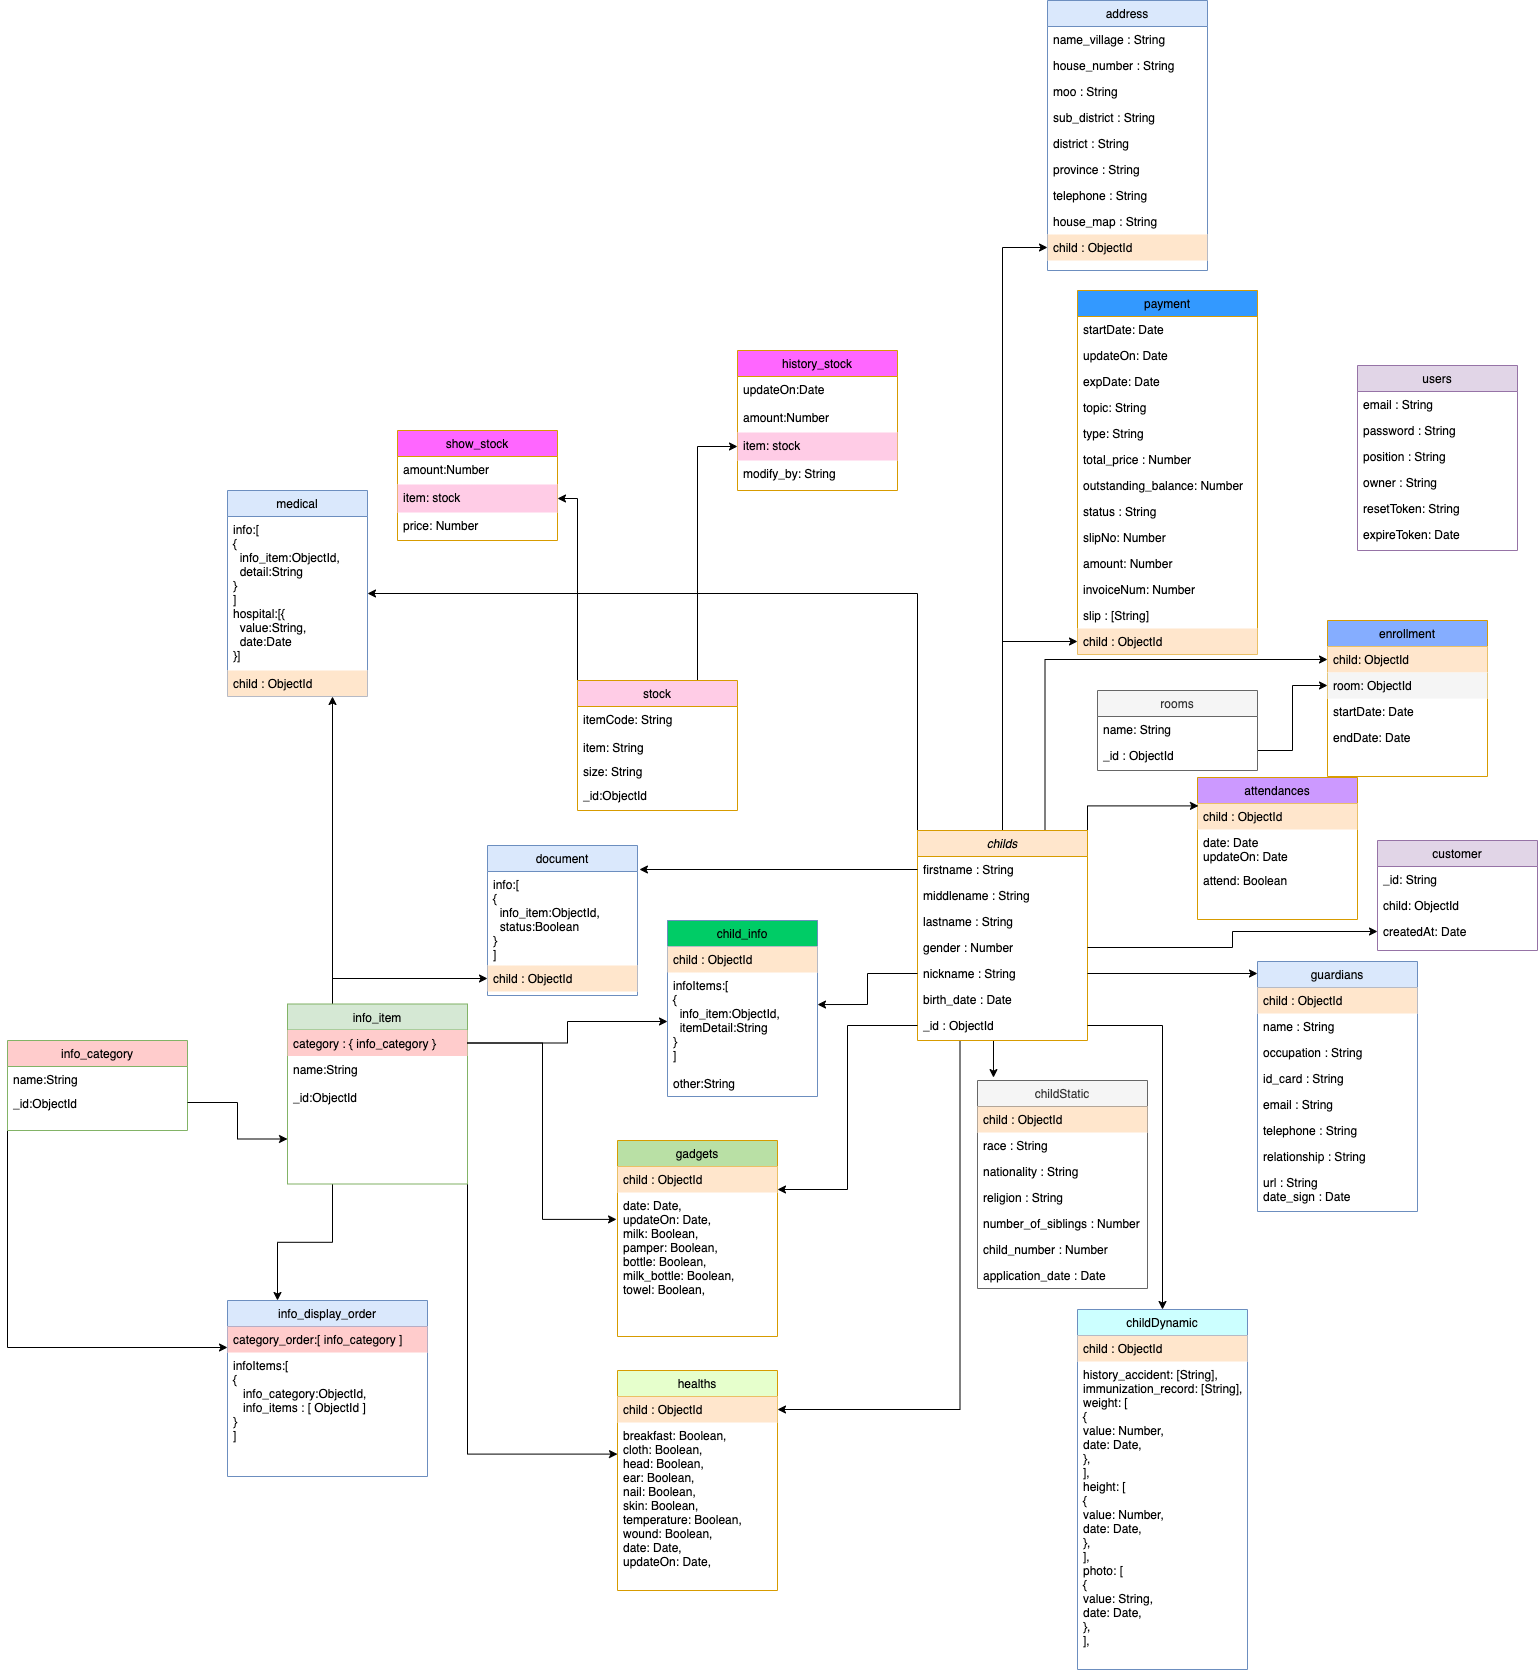
\includegraphics[height=0.9\textheight]{images/NurseryDiagram.png}
    \end{center}
  \caption{แผนภาพแสดงรายละเอียดฐานข้อมูลของระบบ}
  \label{fig:DatabaseDiagram}
\end{figure}
\end{landscape}

\begin{figure}
  \begin{center}
    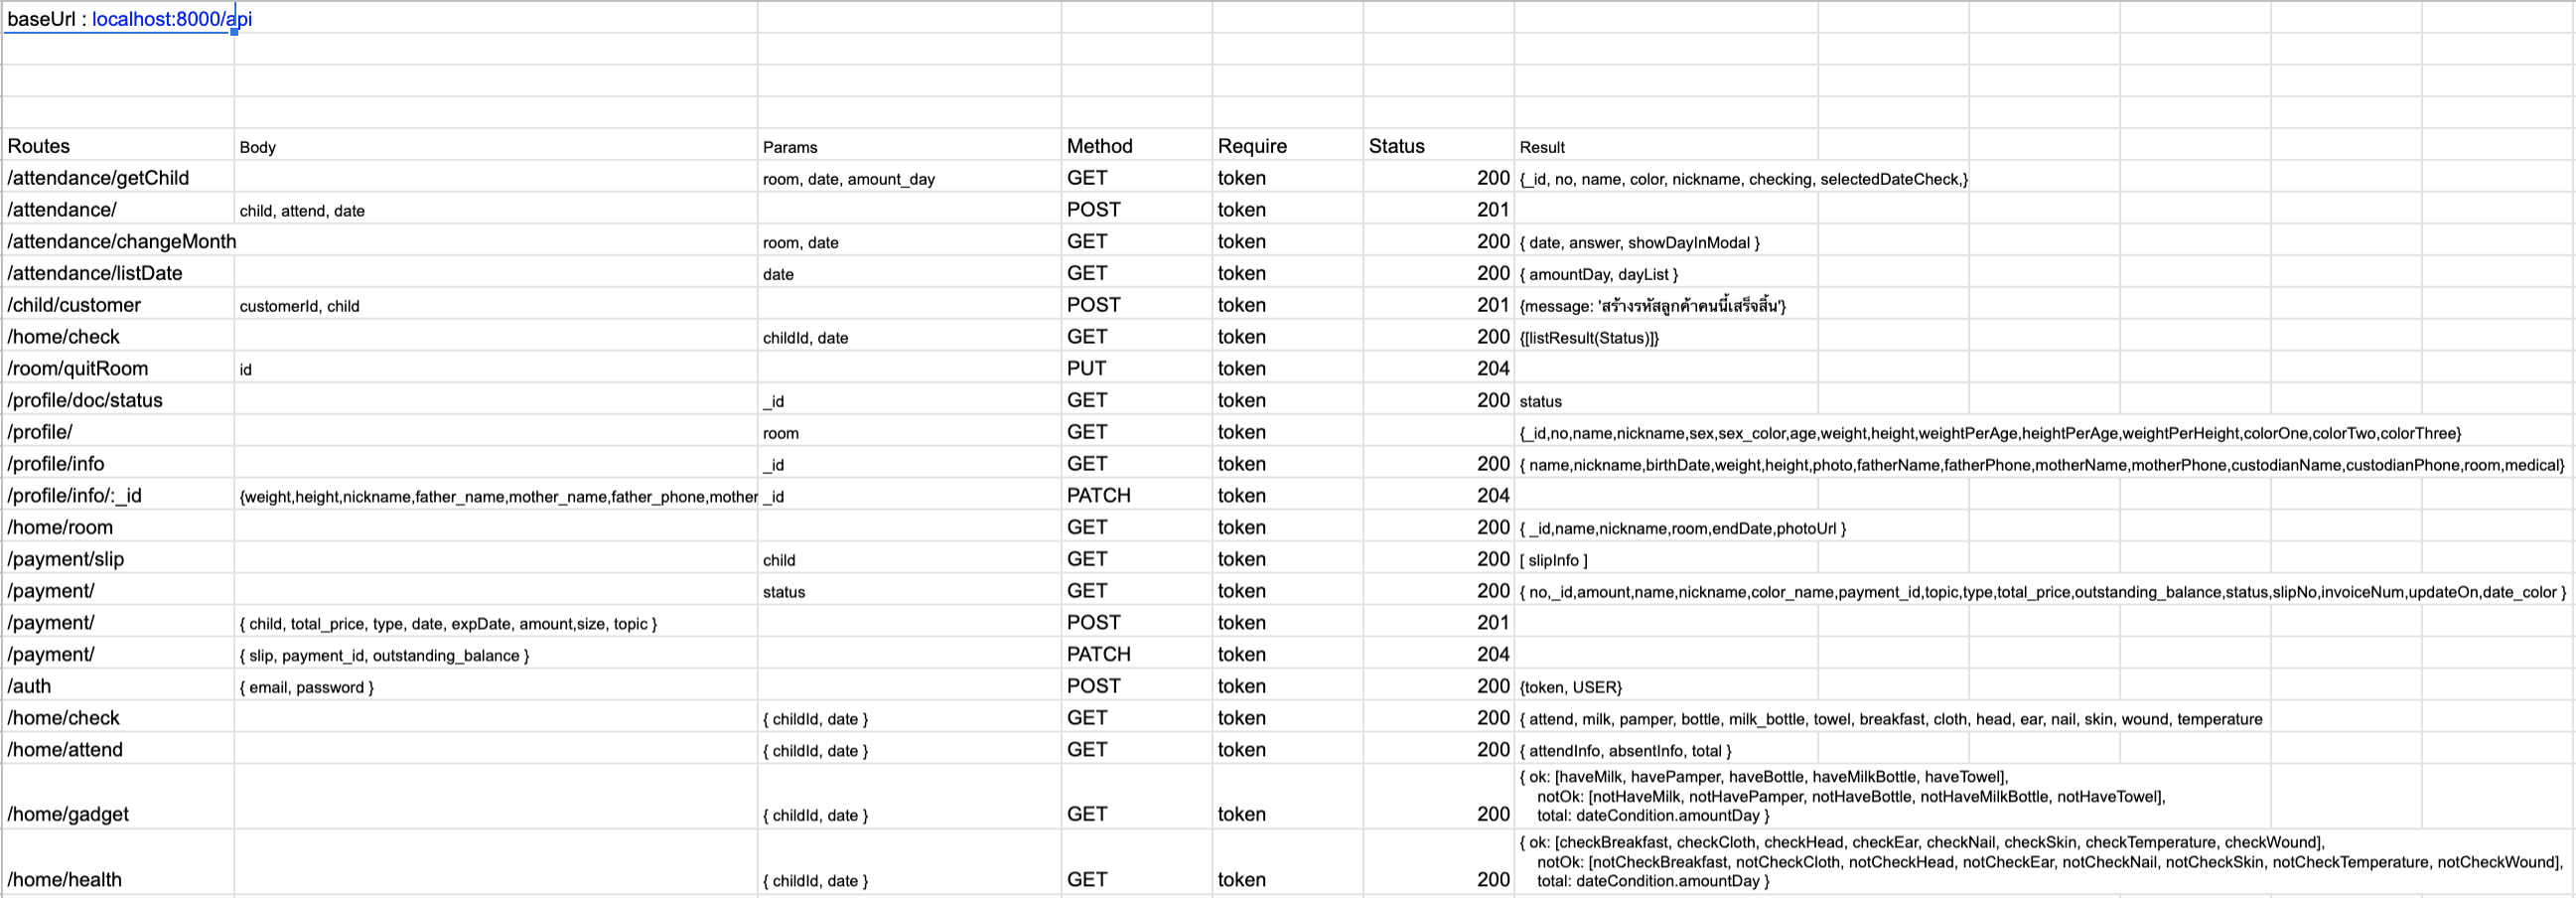
\includegraphics[width=\linewidth]{images/ApiDocOne.png}
  \end{center}
  \caption[Poem]{ApiDocs1}
  \label{fig:ApiDocs1}
\end{figure}

\begin{figure}
  \begin{center}
    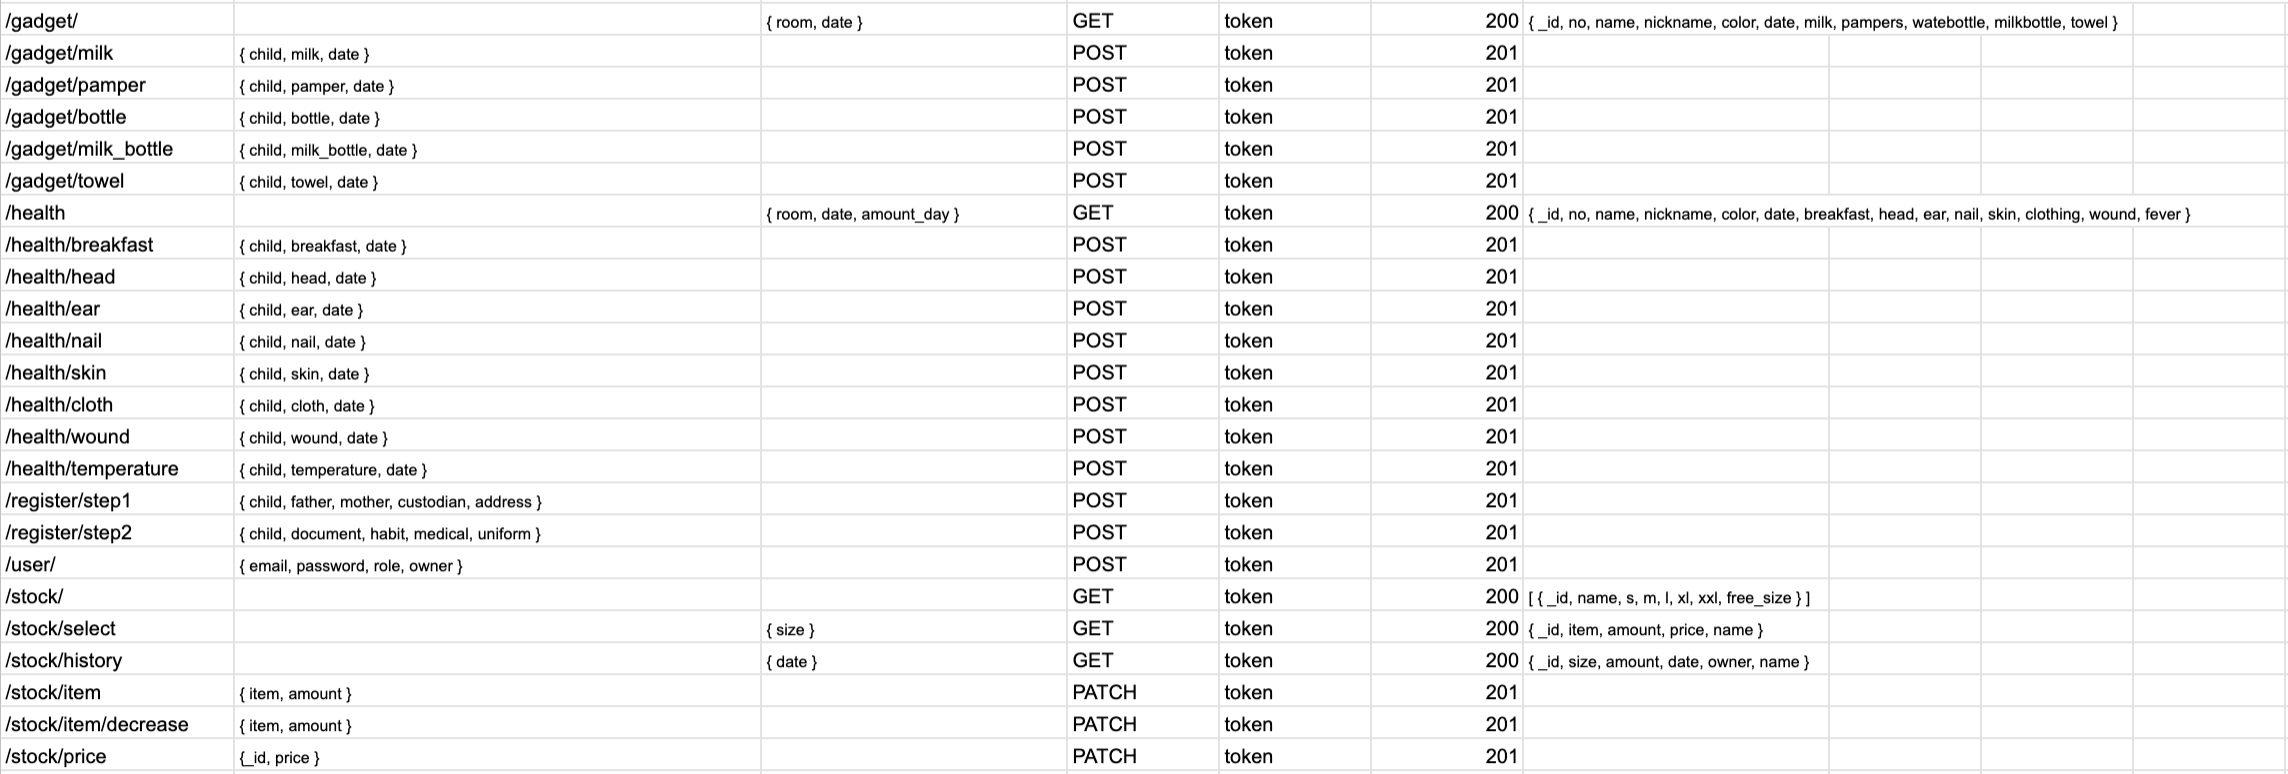
\includegraphics[width=\linewidth]{images/ApiDocTwo.png}
  \end{center}
  \caption[Poem]{ApiDocs2}
  \label{fig:ApiDocs2}
\end{figure}

\begin{figure}
  \begin{center}
  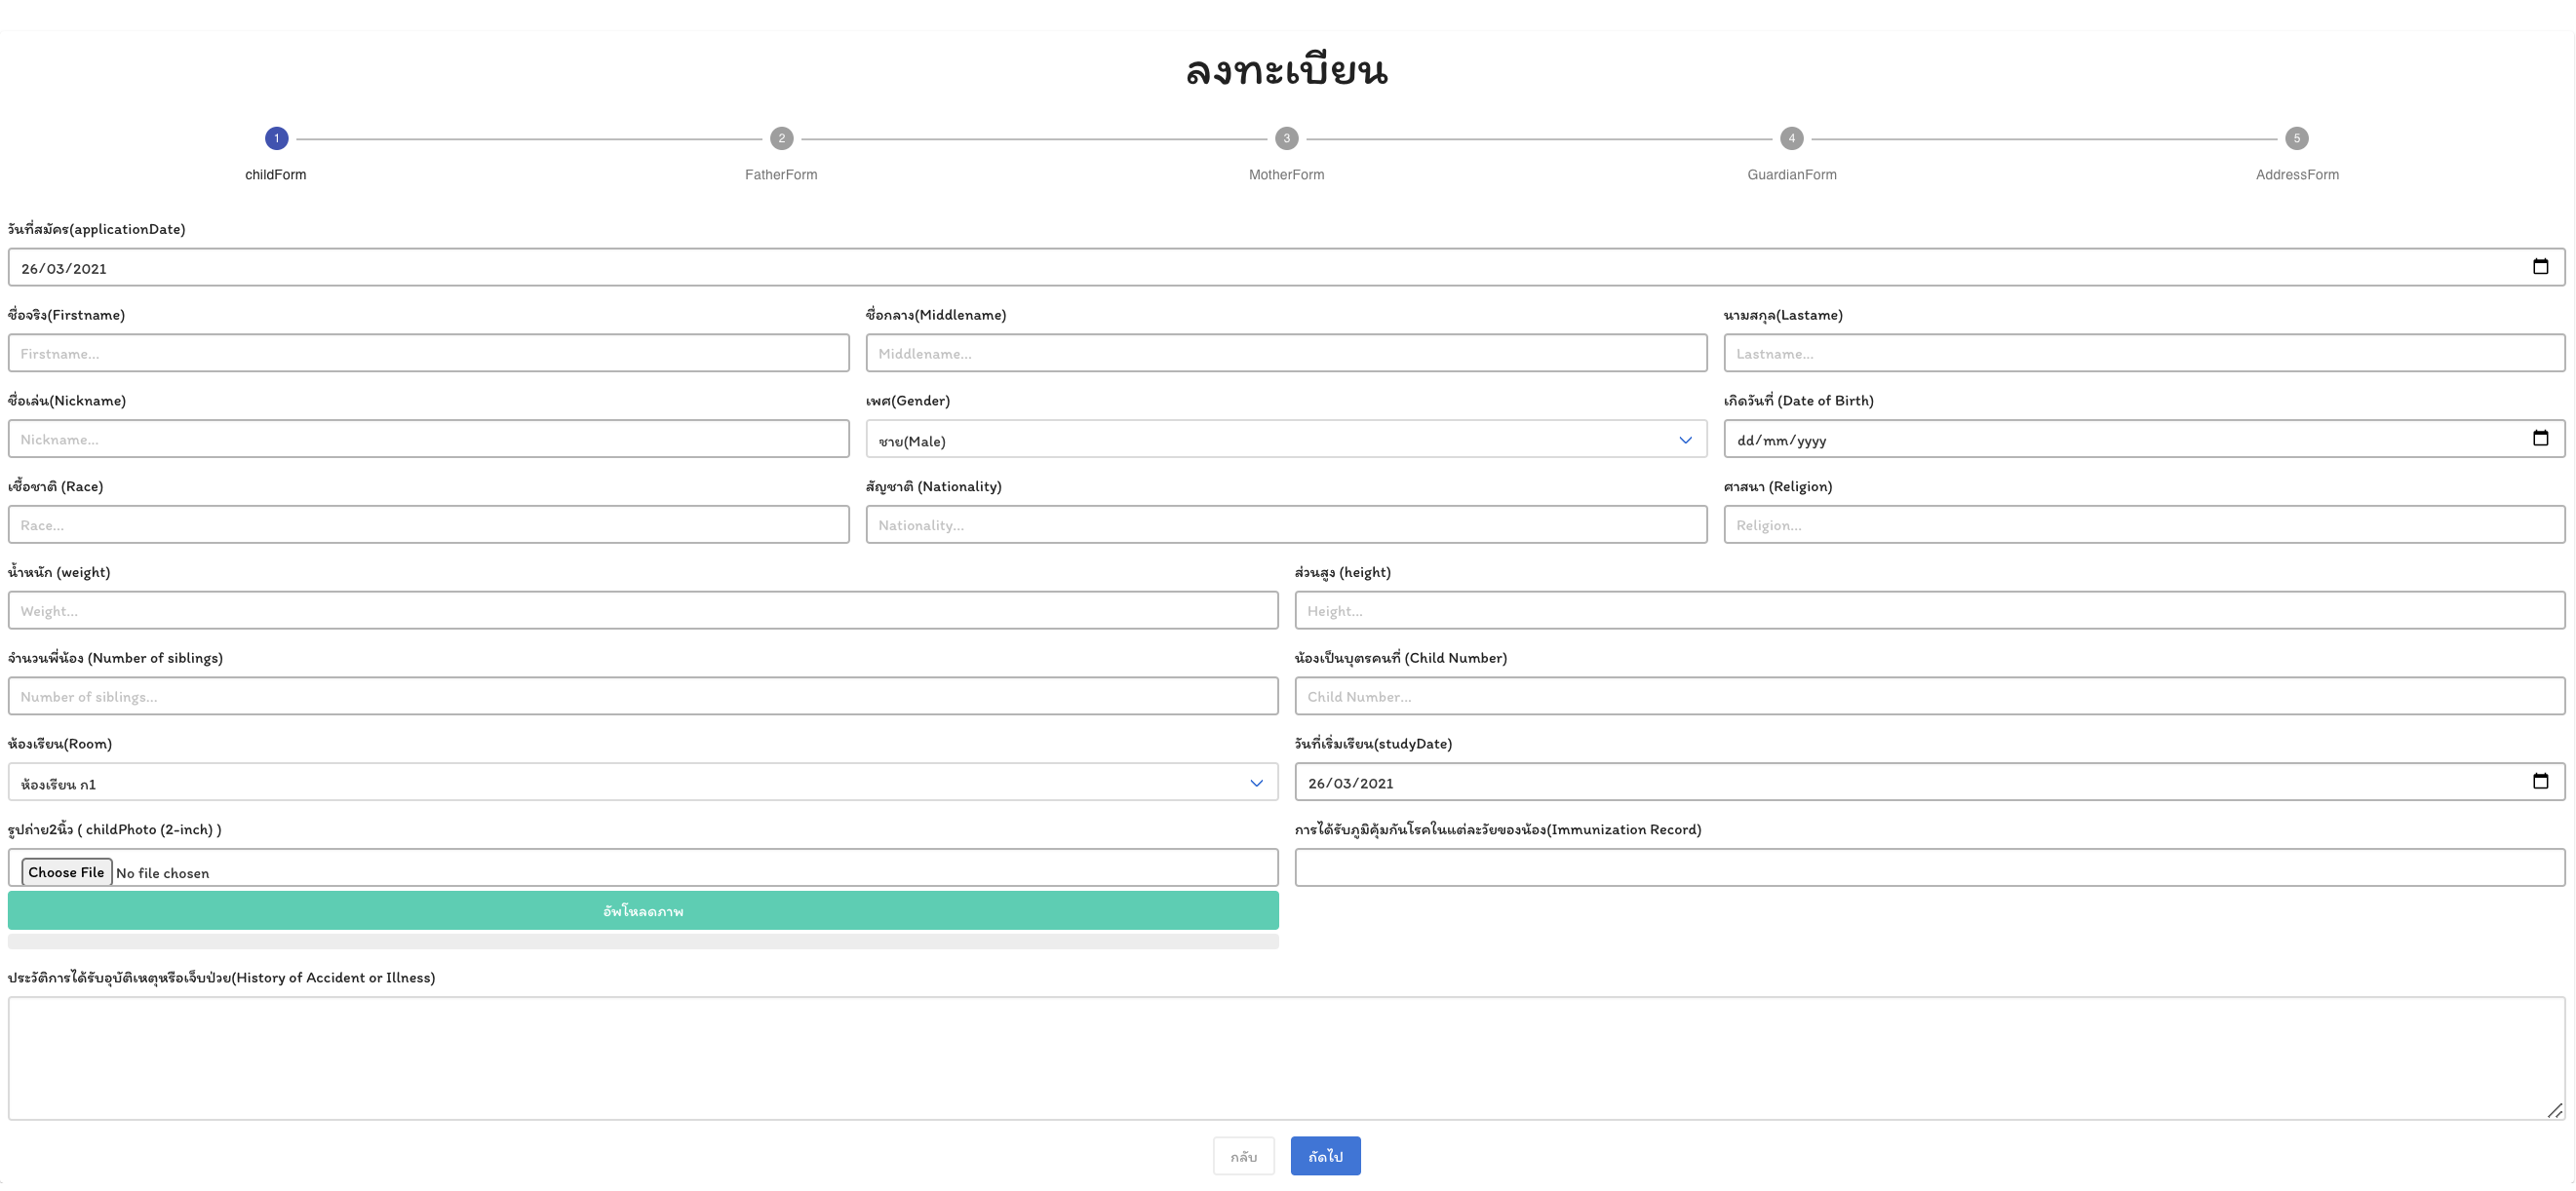
\includegraphics[width=\linewidth]{images/RegisterForm.png}
  \end{center}
  \caption[Poem]{Register Form}
  \label{fig:register}
  \end{figure}

\begin{figure}
  \begin{center}
  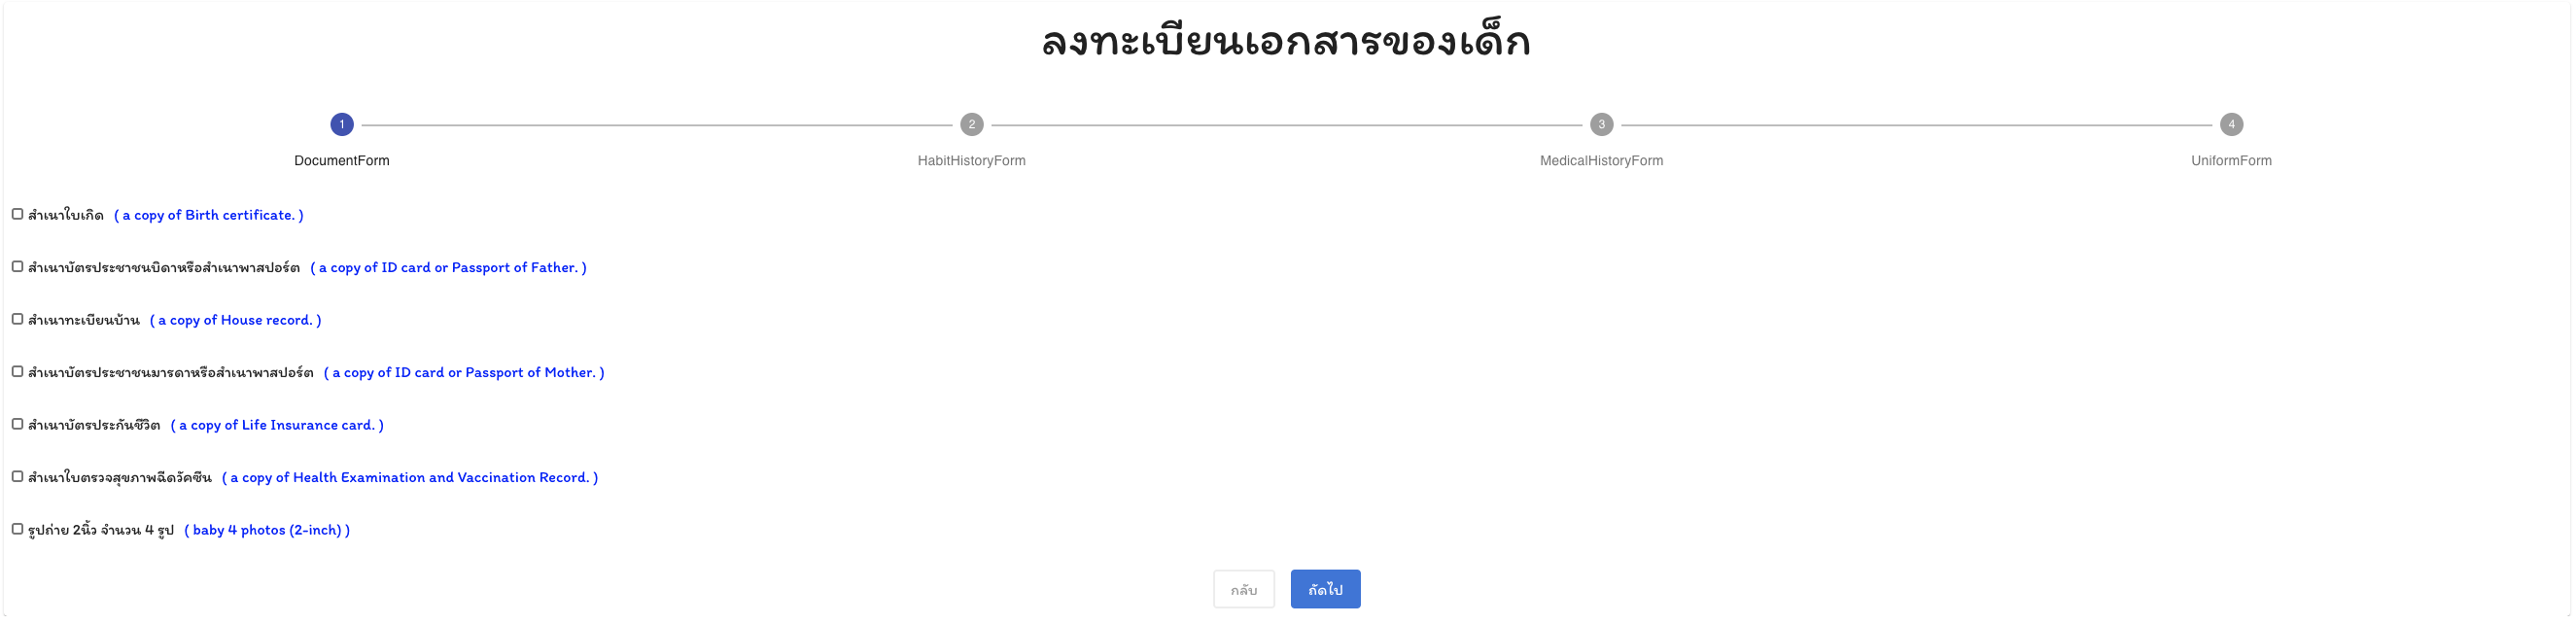
\includegraphics[width=\linewidth]{images/DocForm.png}
  \end{center}
  \caption[Poem]{DocForm}
  \label{fig:docForm}
  \end{figure}

\begin{figure}
  \begin{center}
  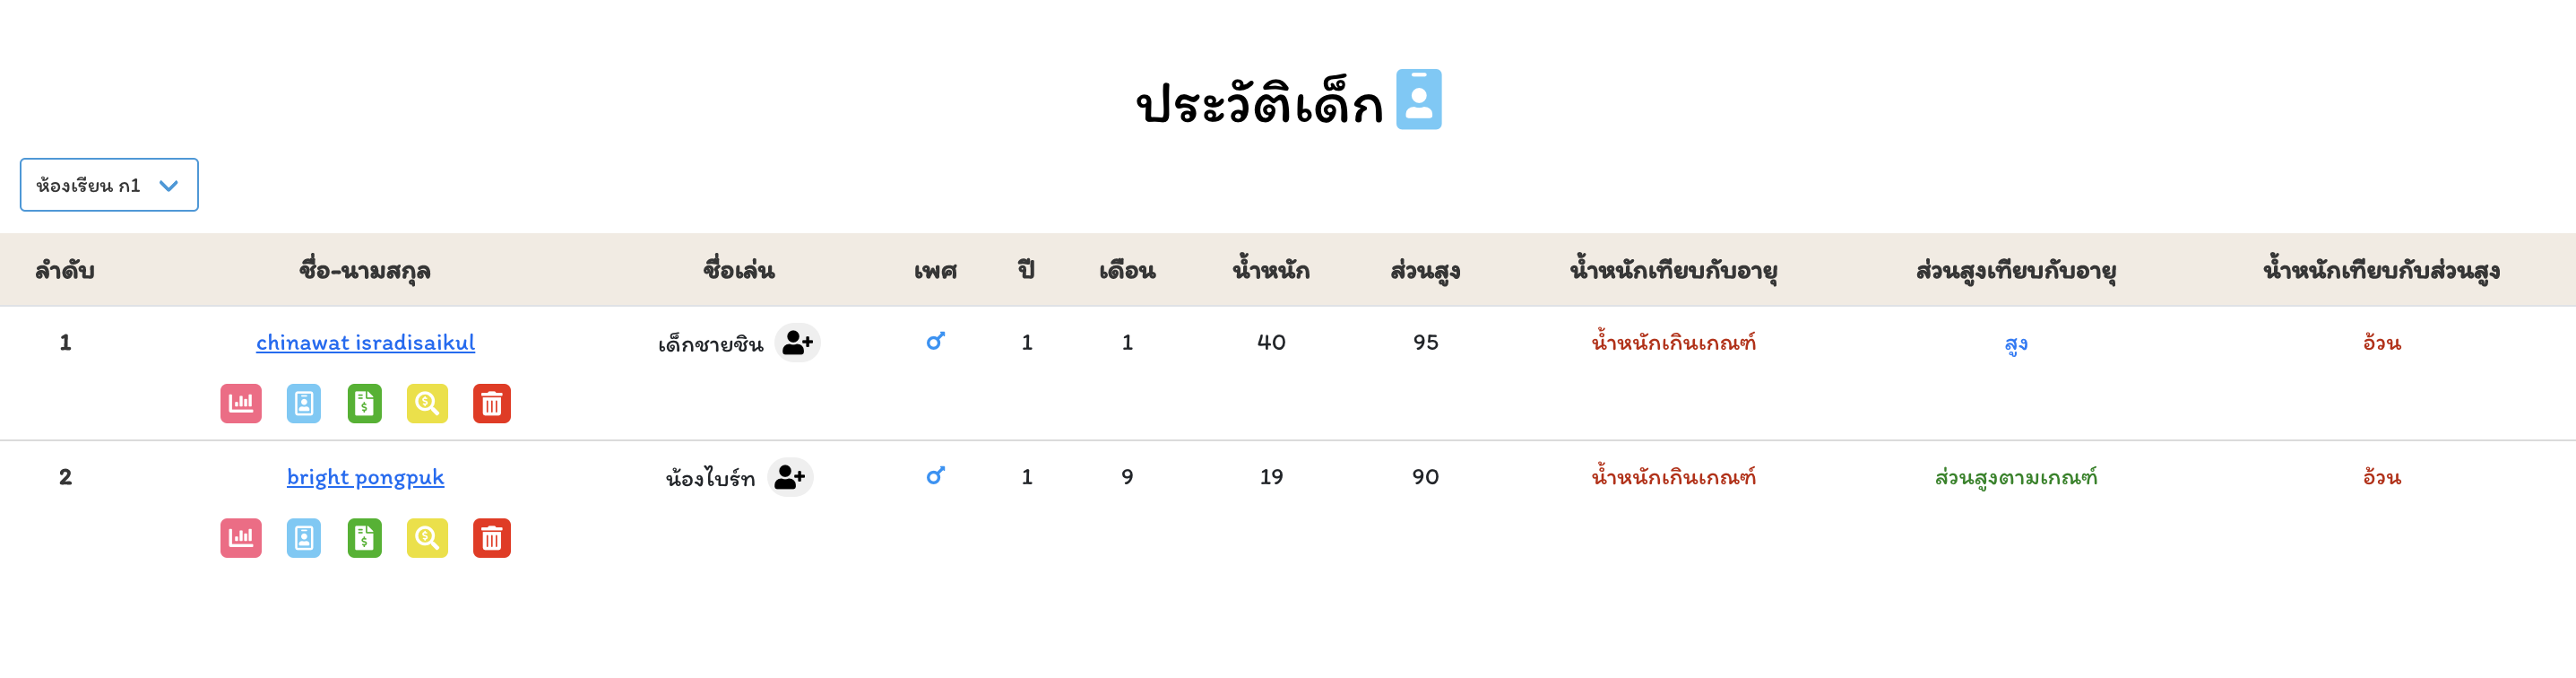
\includegraphics[width=\linewidth]{images/Profile.png}
  \end{center}
  \caption[Poem]{Profile Page}
  \label{fig:Profile}
  \end{figure}

\begin{figure}
  \begin{center}
  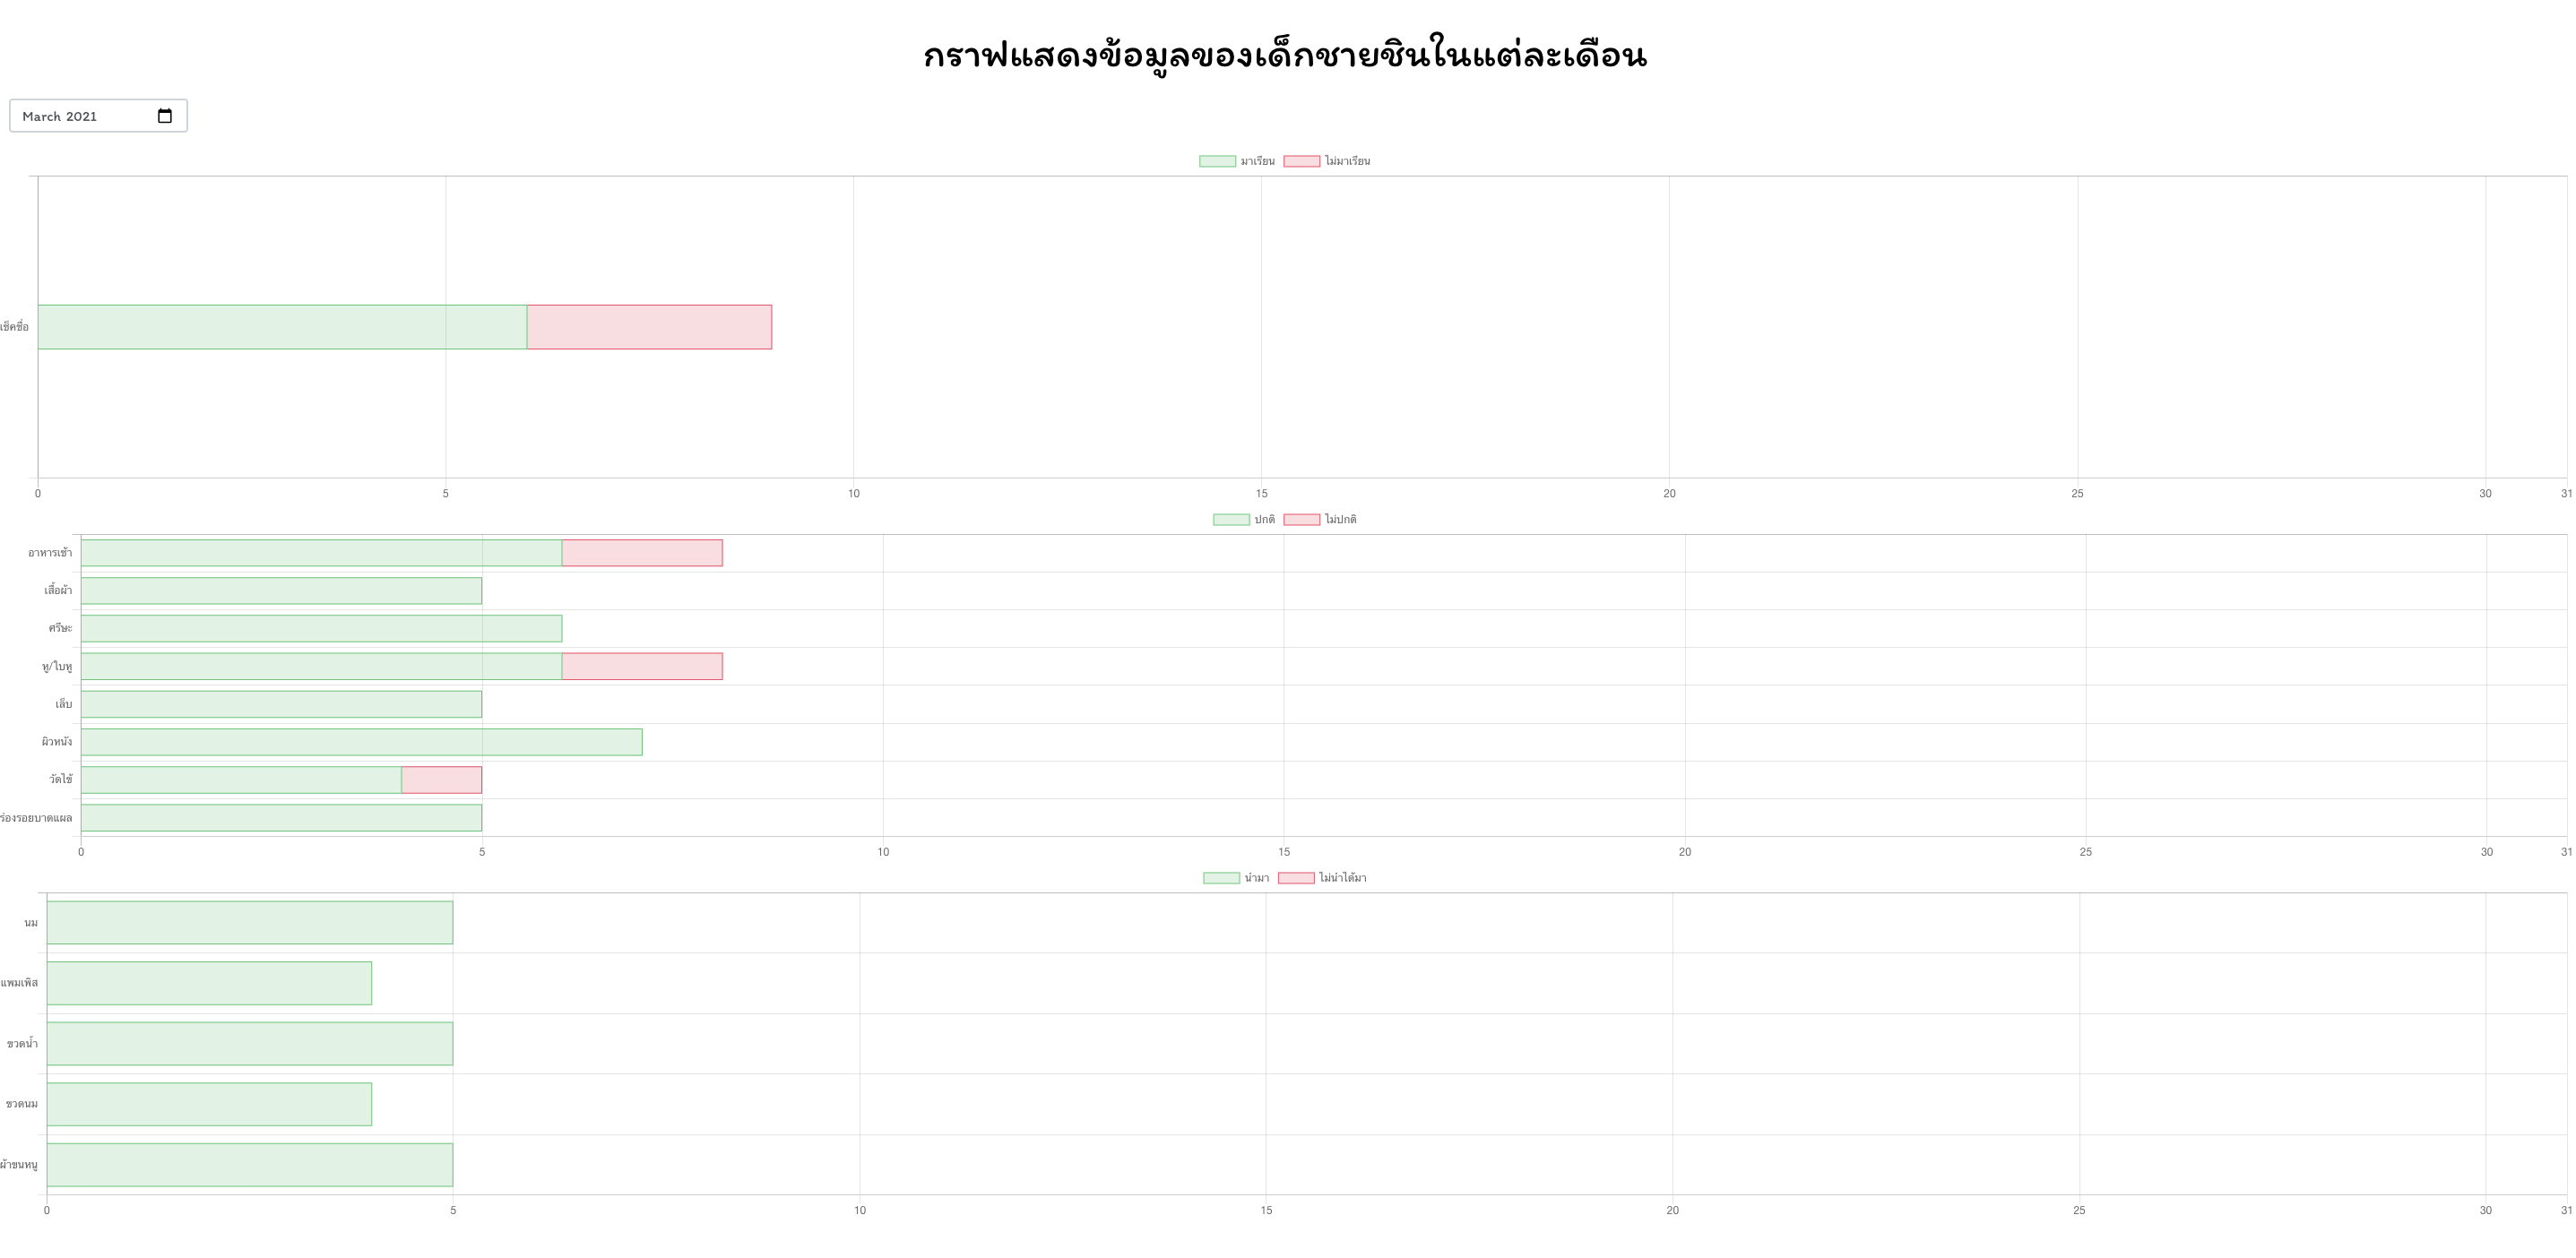
\includegraphics[width=\linewidth]{images/ChartPage.png}
  \end{center}
  \caption[Poem]{Show Chart Page}
  \label{fig:ChartPage}
  \end{figure}
  
\begin{figure}
  \begin{center}
  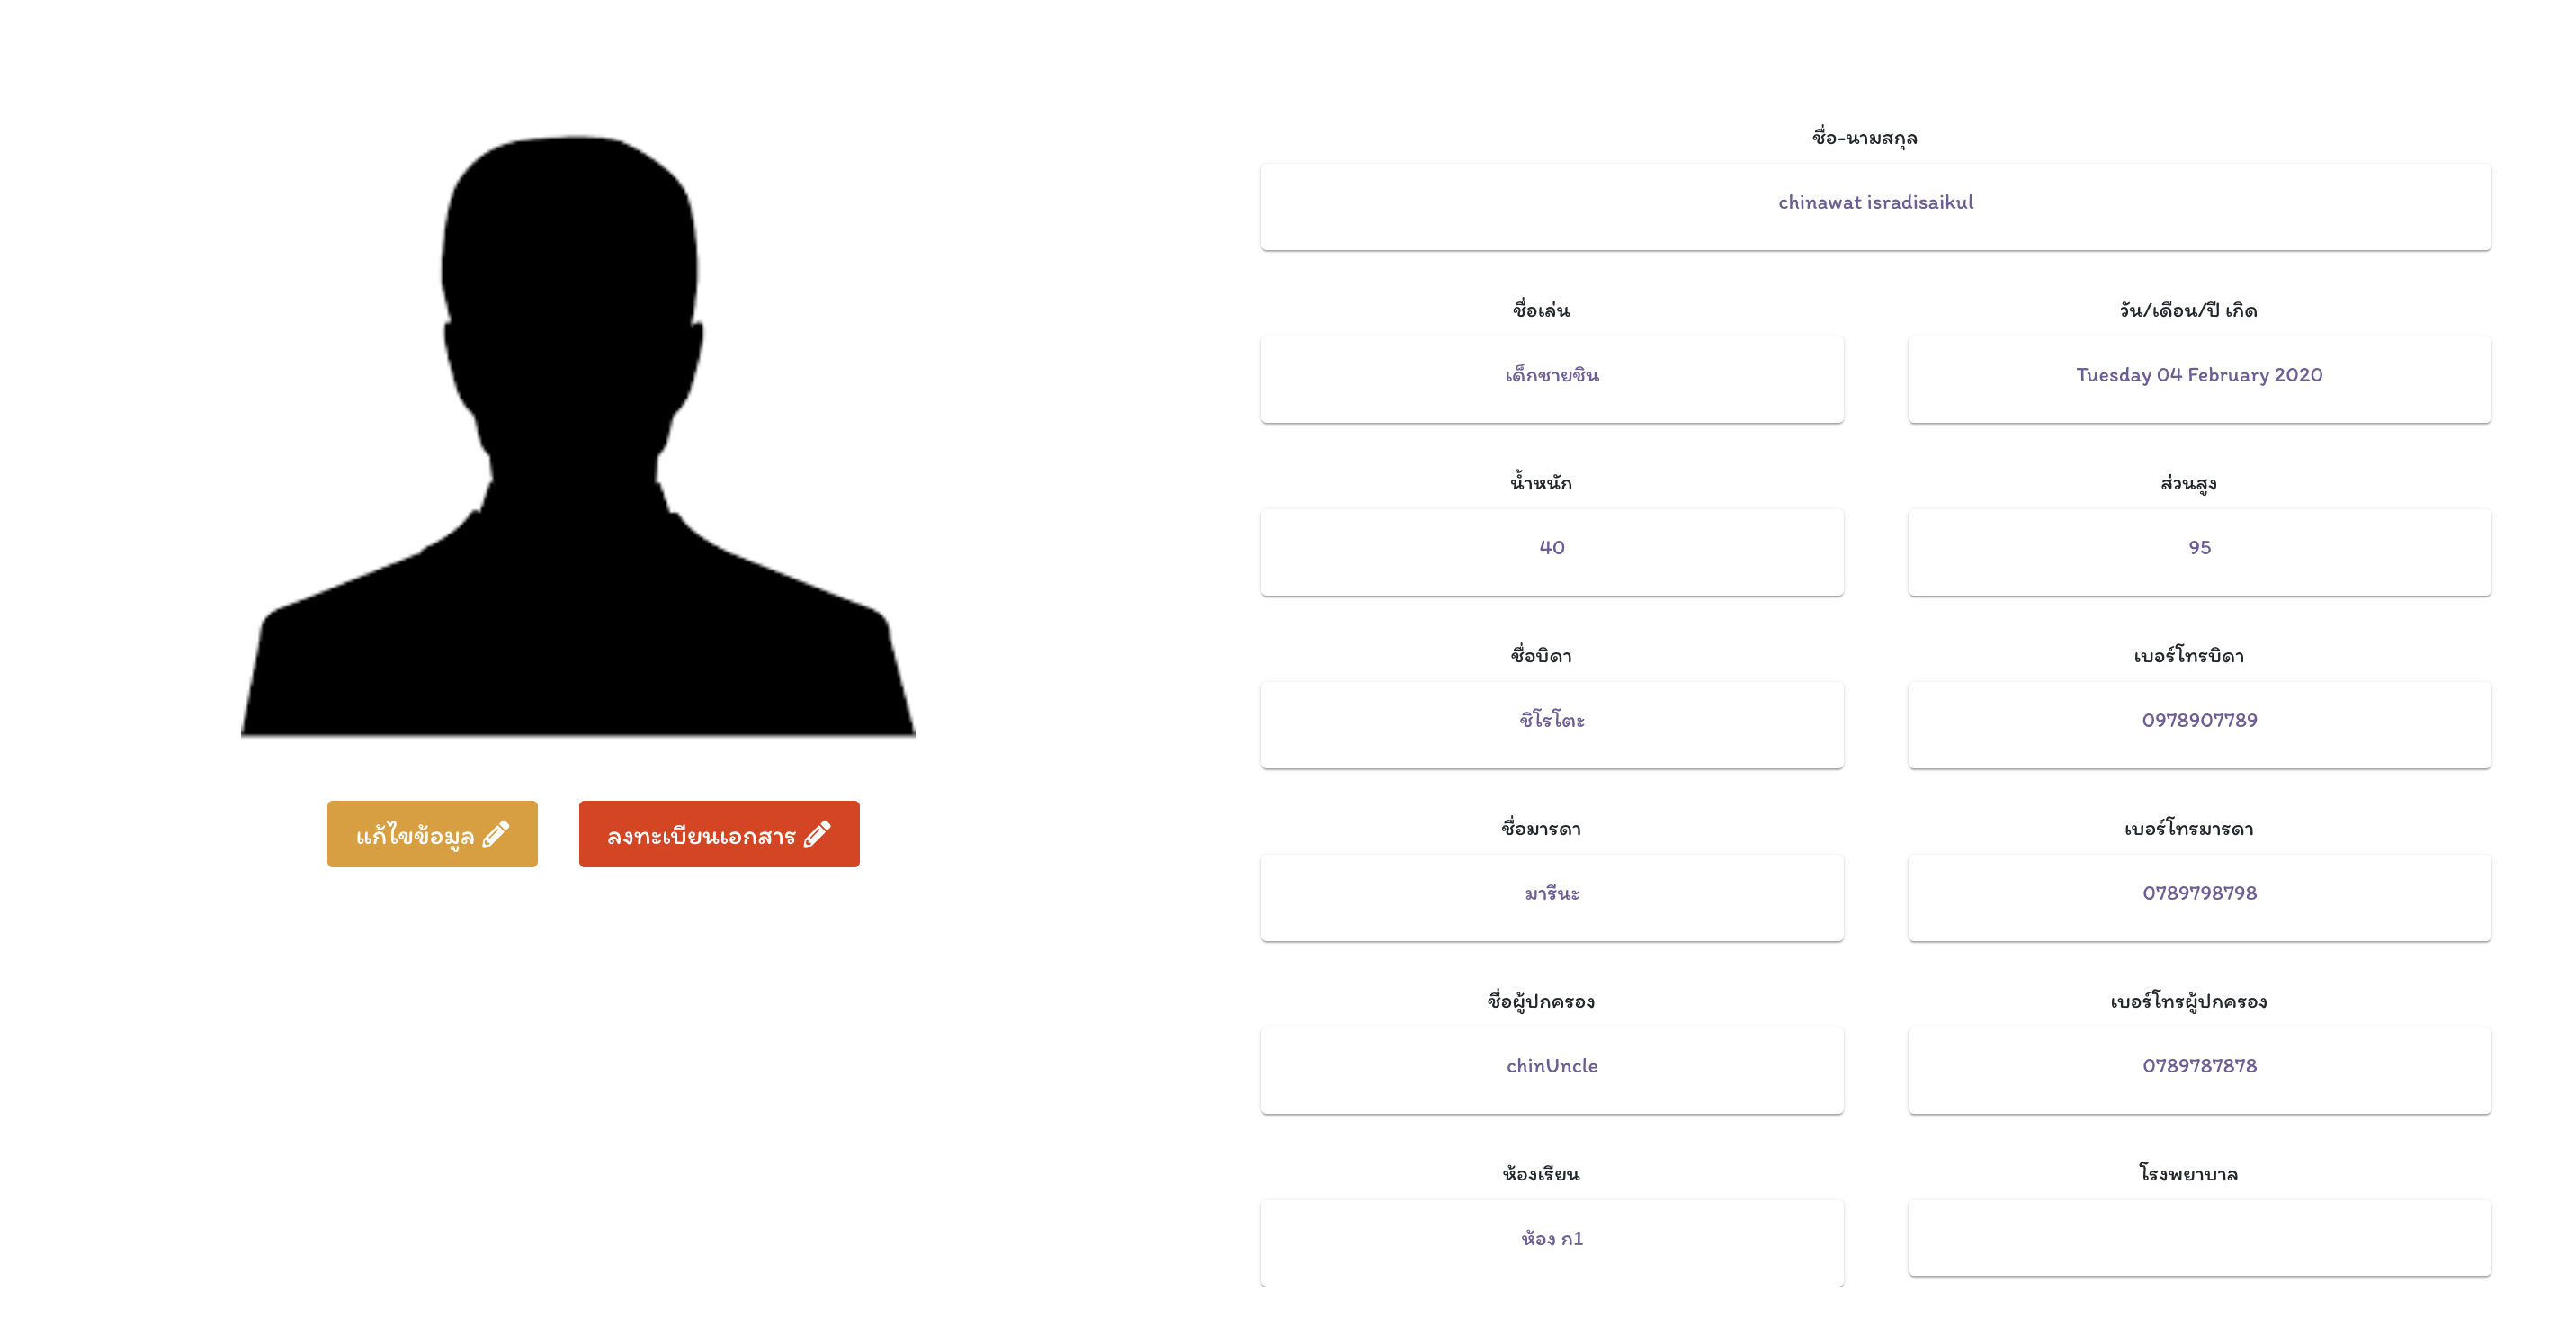
\includegraphics[width=\linewidth]{images/ProfileInfo.png}
  \end{center}
  \caption[Poem]{ProfileInfo Page}
  \label{fig:ProfileTwo}
  \end{figure}

\begin{figure}
  \begin{center}
  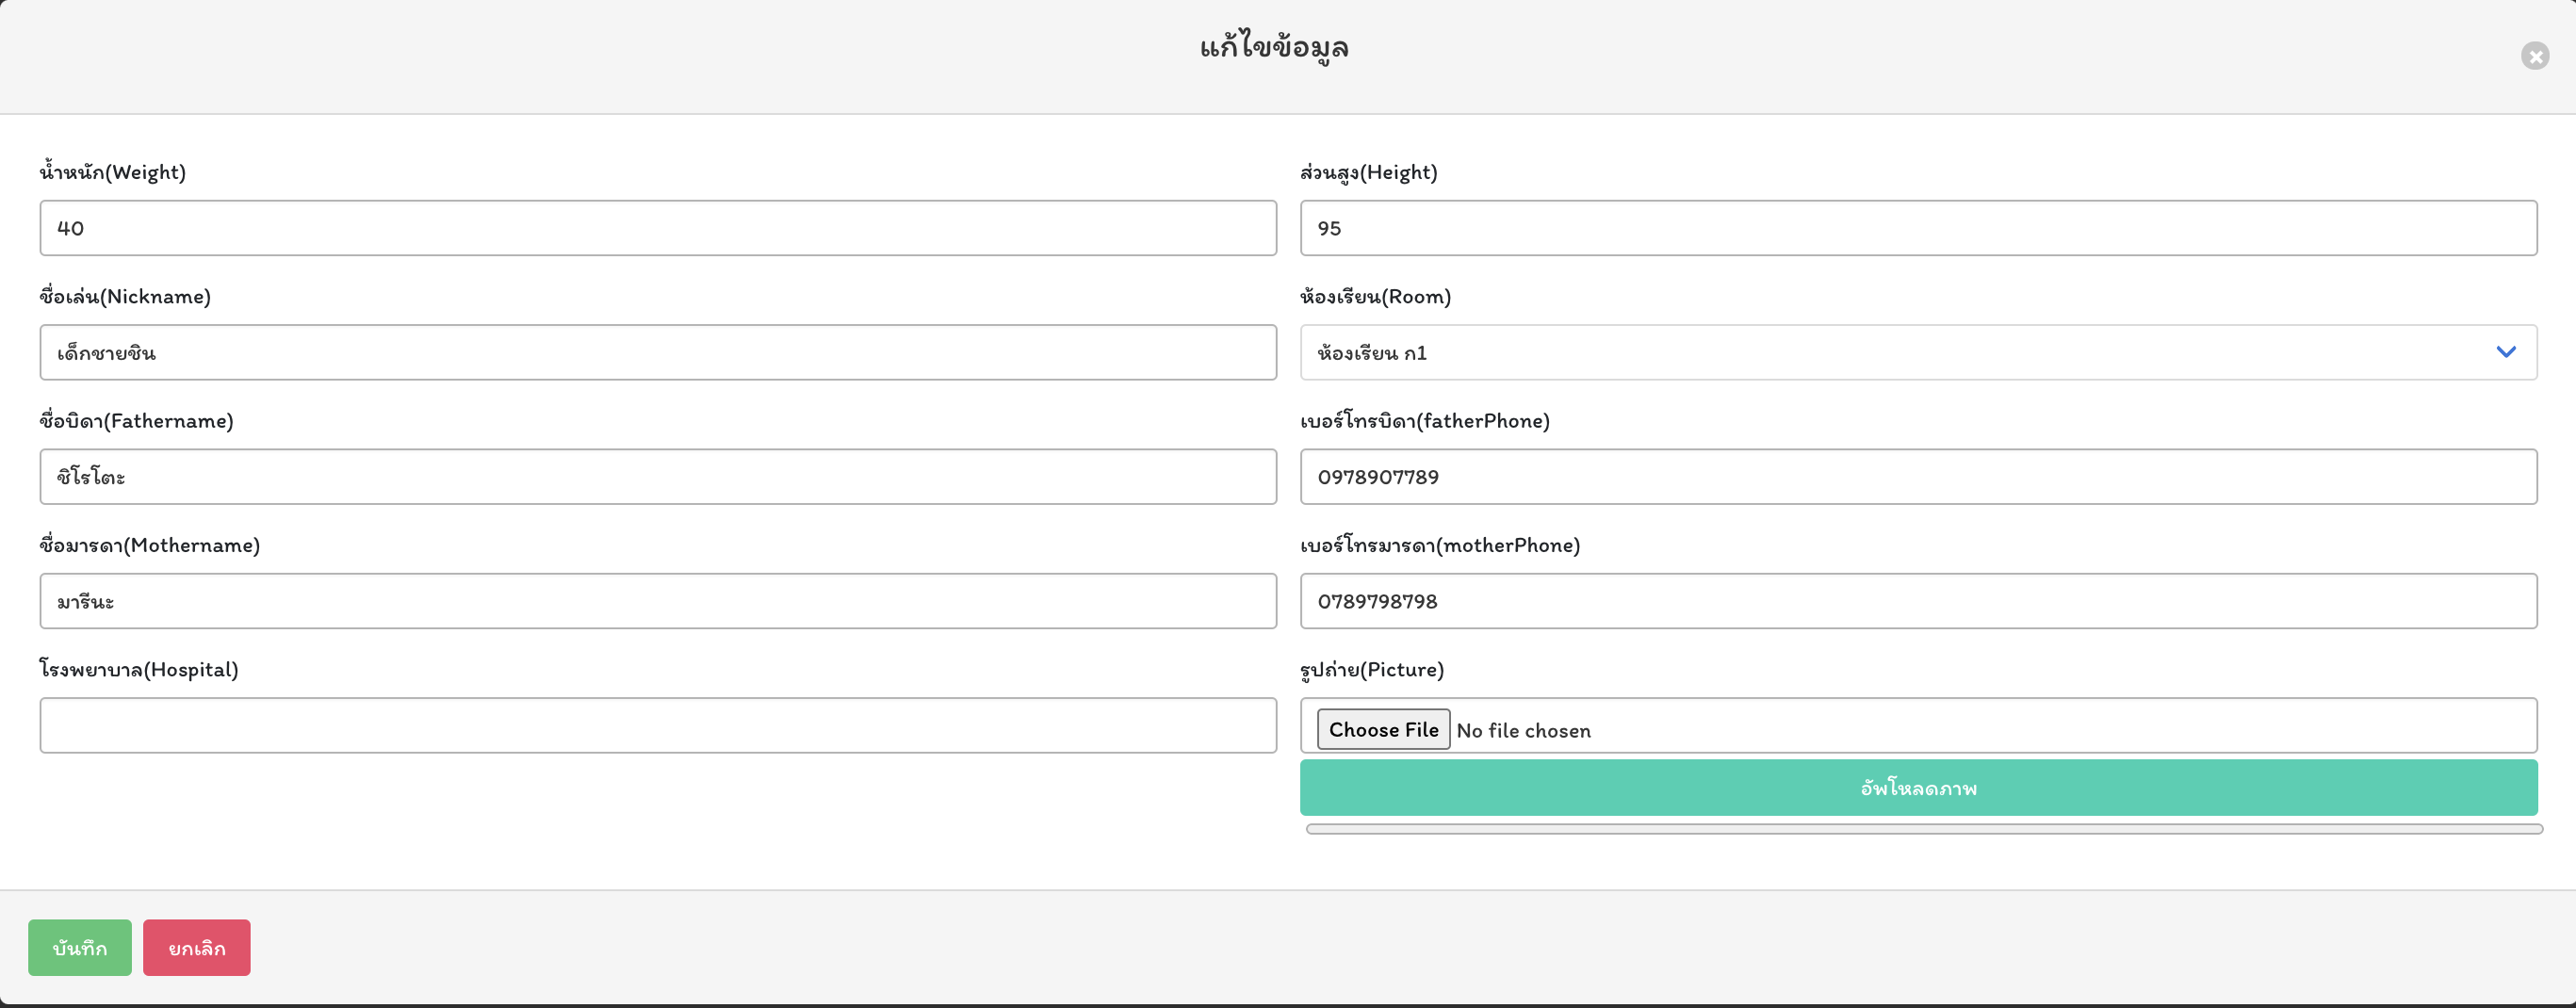
\includegraphics[width=\linewidth]{images/updateProfile.png}
  \end{center}
  \caption[Poem]{Update Profile Modal}
  \label{fig:UpdateProfile}
  \end{figure}
\begin{figure}
  \begin{center}
  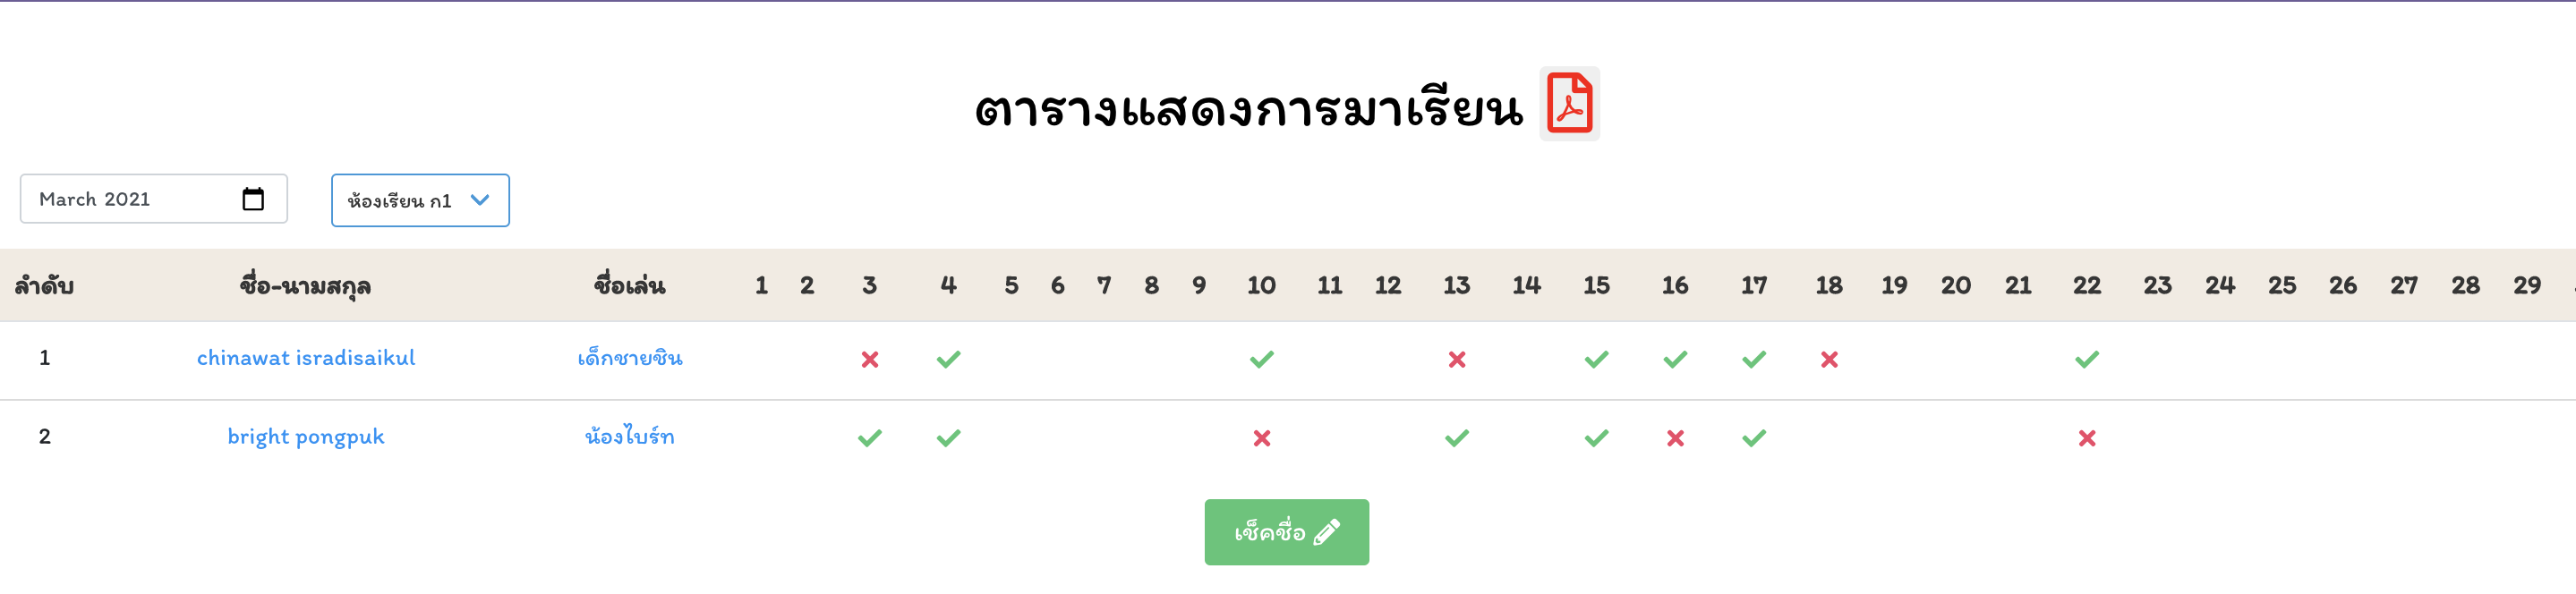
\includegraphics[width=\linewidth]{images/Attendance.png}
  \end{center}
  \caption[Poem]{Attendance Page}
  \label{fig:Attendance}
  \end{figure}

\begin{figure}
  \begin{center}
  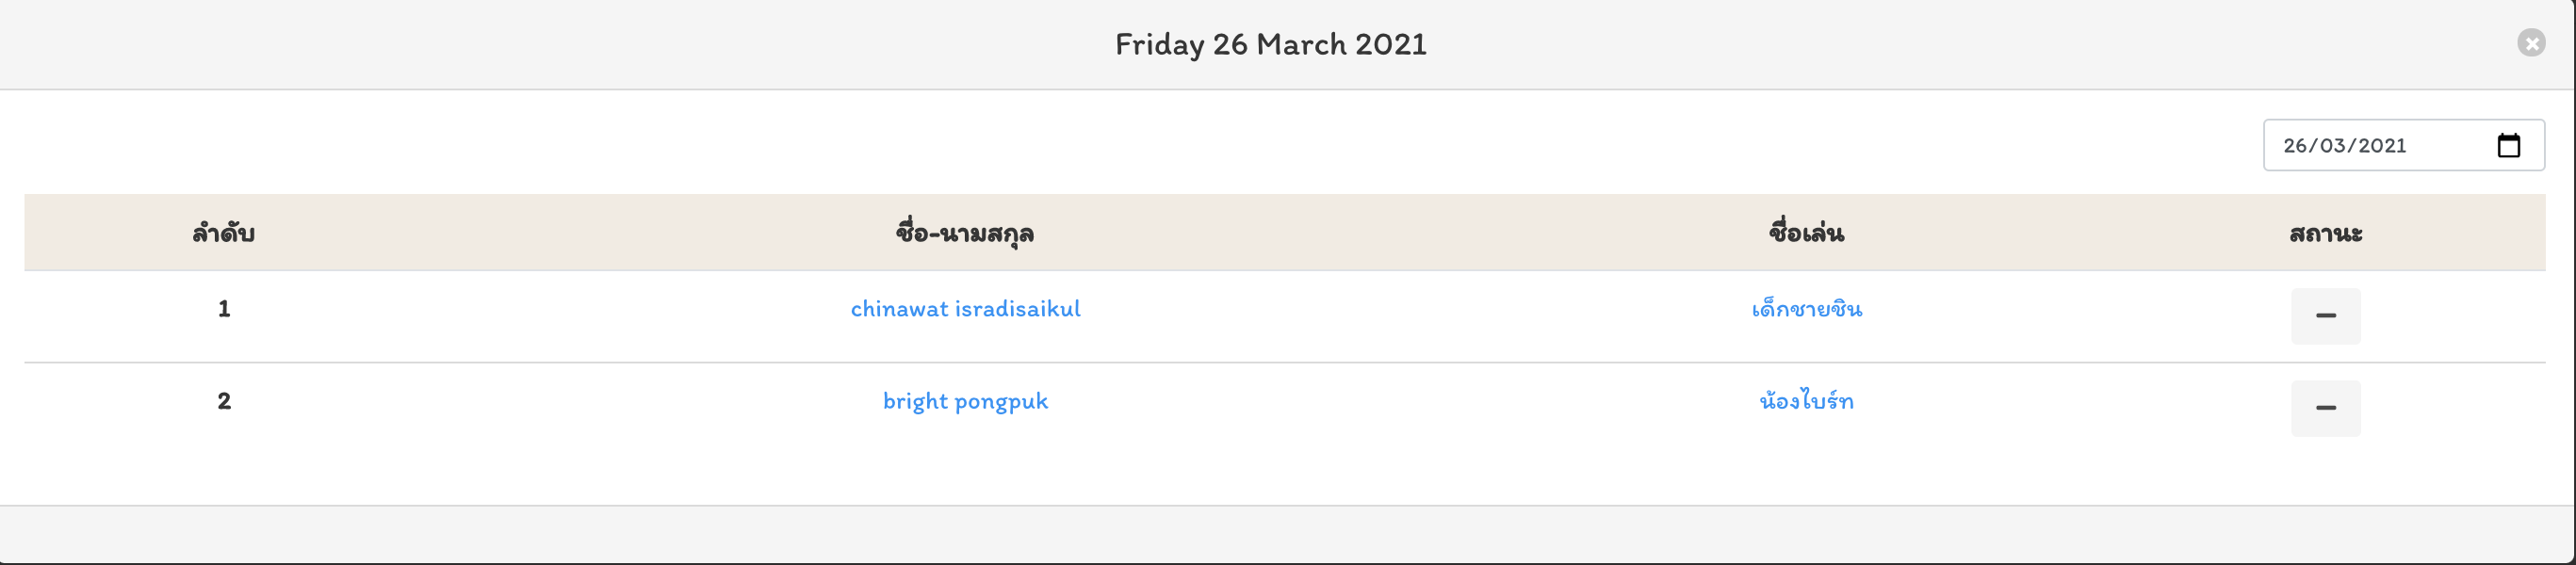
\includegraphics[width=\linewidth]{images/checkAttendance.png}
  \end{center}
  \caption[Poem]{Attendance Checking Modal}
  \label{fig:CheckAttendance}
  \end{figure}

\begin{figure}
  \begin{center}
  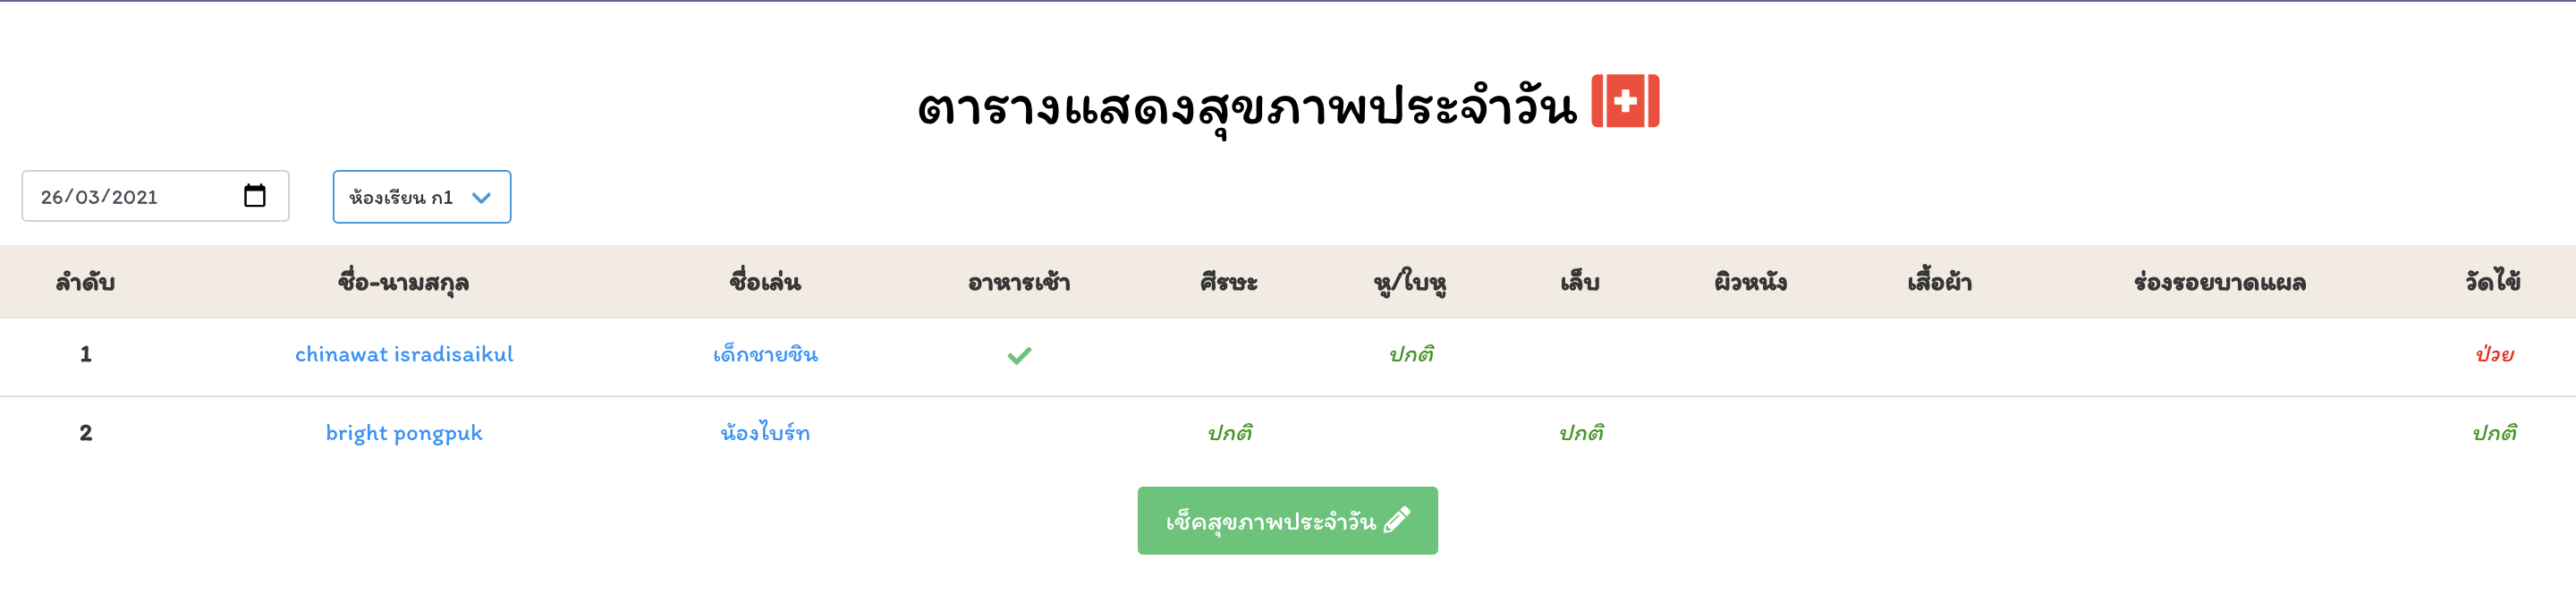
\includegraphics[width=\linewidth]{images/Health.png}
  \end{center}
  \caption[Poem]{Health Page}
  \label{fig:Health}
  \end{figure}

\begin{figure}
  \begin{center}
  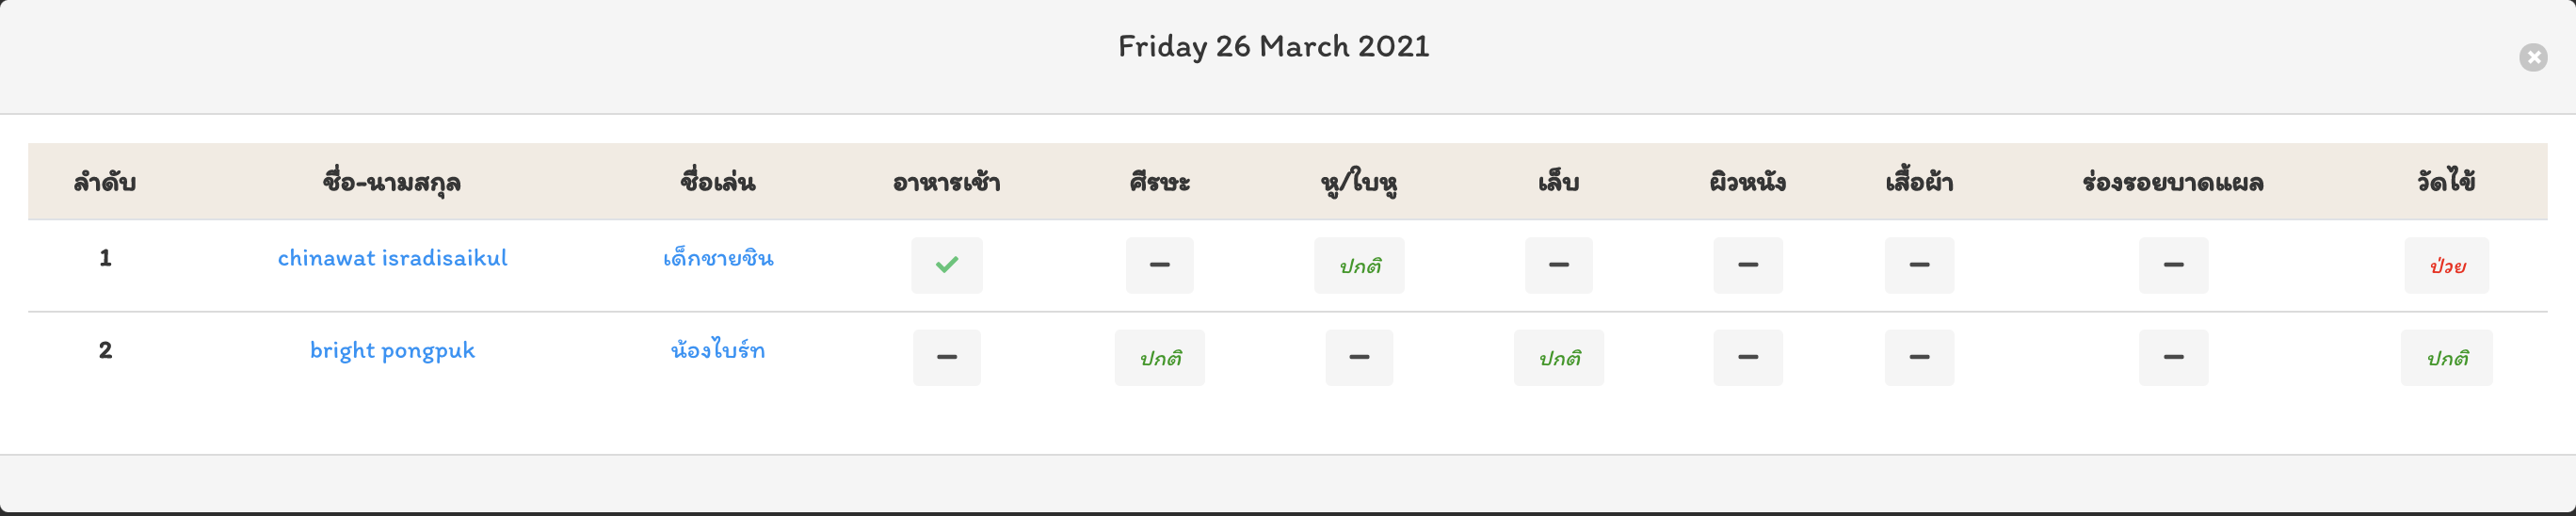
\includegraphics[width=\linewidth]{images/checkHealth.png}
  \end{center}
  \caption[Poem]{Health Checking Modal}
  \label{fig:CheckHealth}
  \end{figure}

\begin{figure}
  \begin{center}
  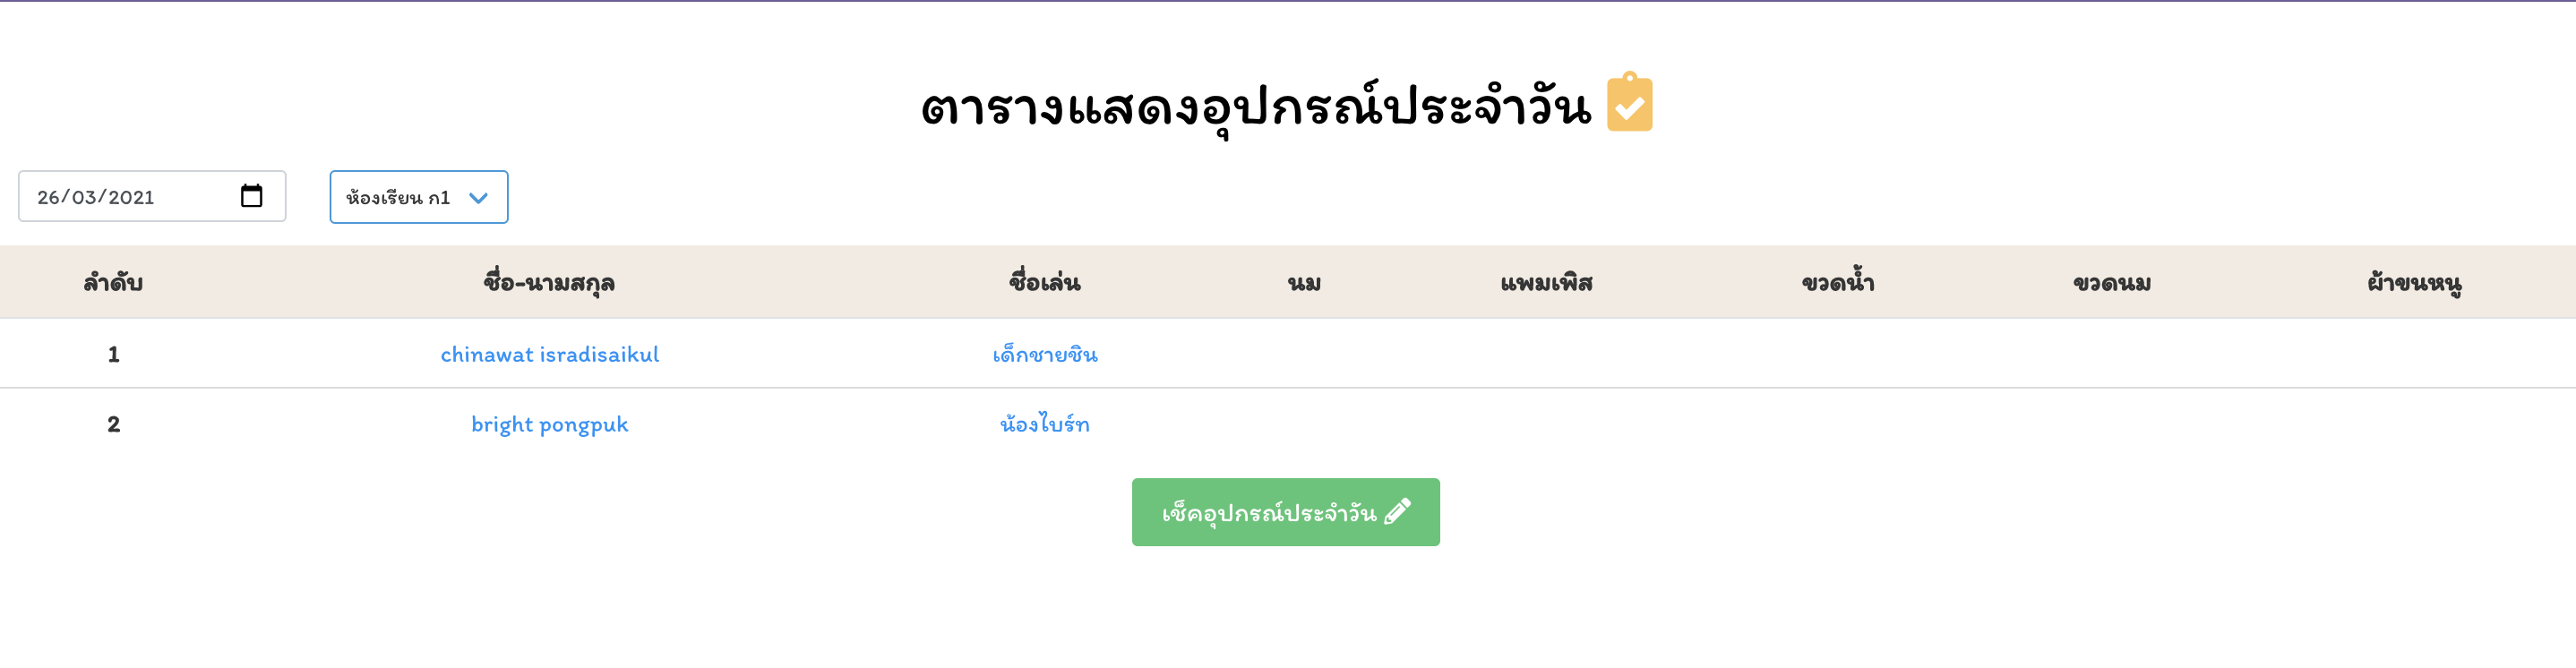
\includegraphics[width=\linewidth]{images/Gadget.png}
  \end{center}
  \caption[Poem]{Gadget Page}
  \label{fig:Gadget}
  \end{figure}

\begin{figure}
  \begin{center}
  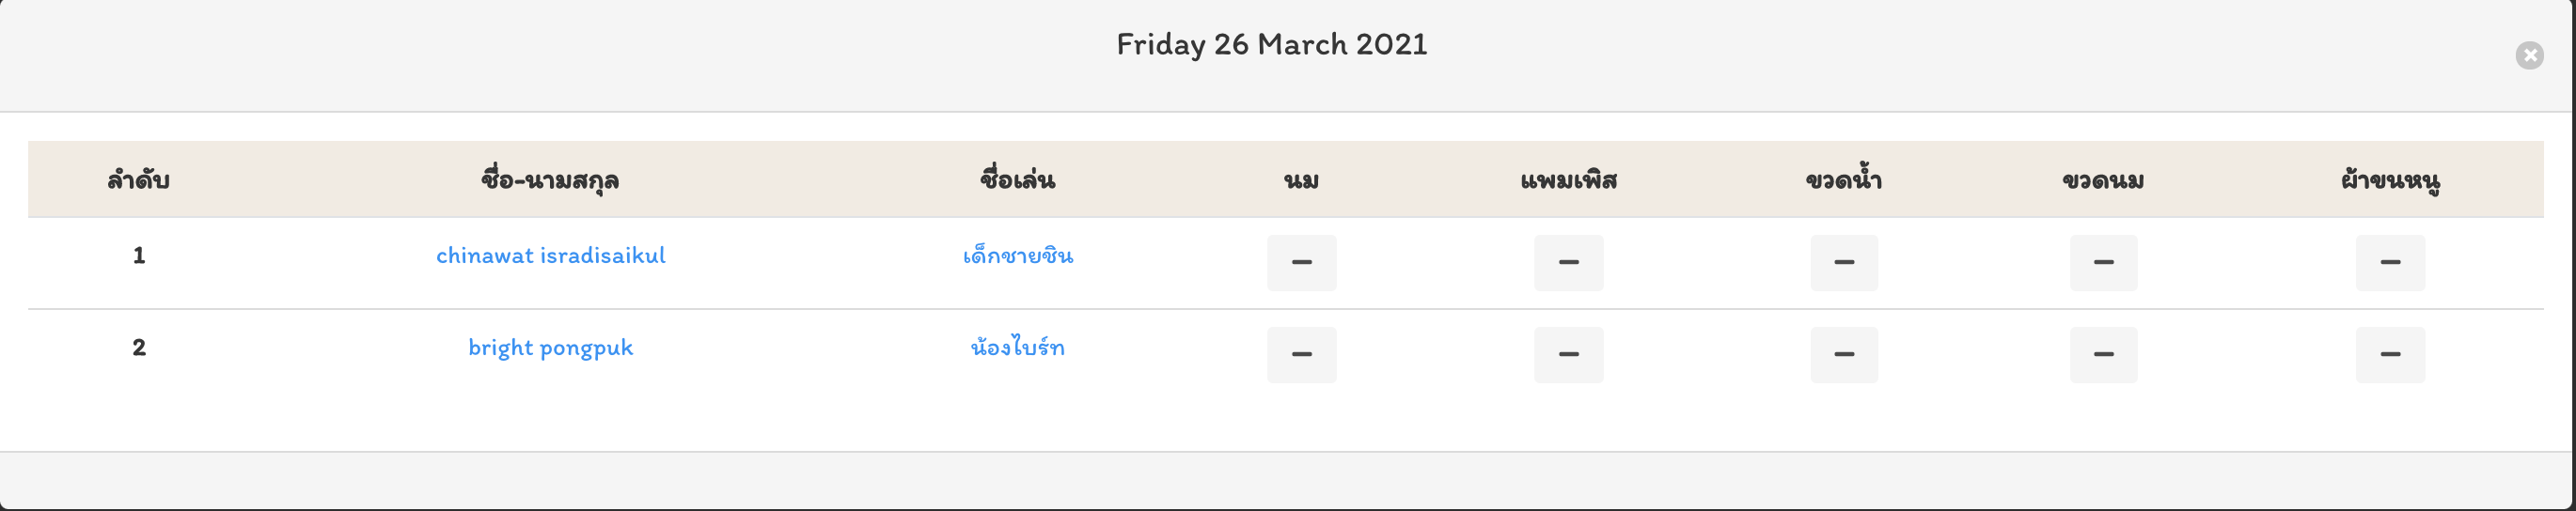
\includegraphics[width=\linewidth]{images/checkGadget.png}
  \end{center}
  \caption[Poem]{Gadget Checking Modal}
  \label{fig:CheckGadget}
  \end{figure}

\begin{figure}
  \begin{center}
  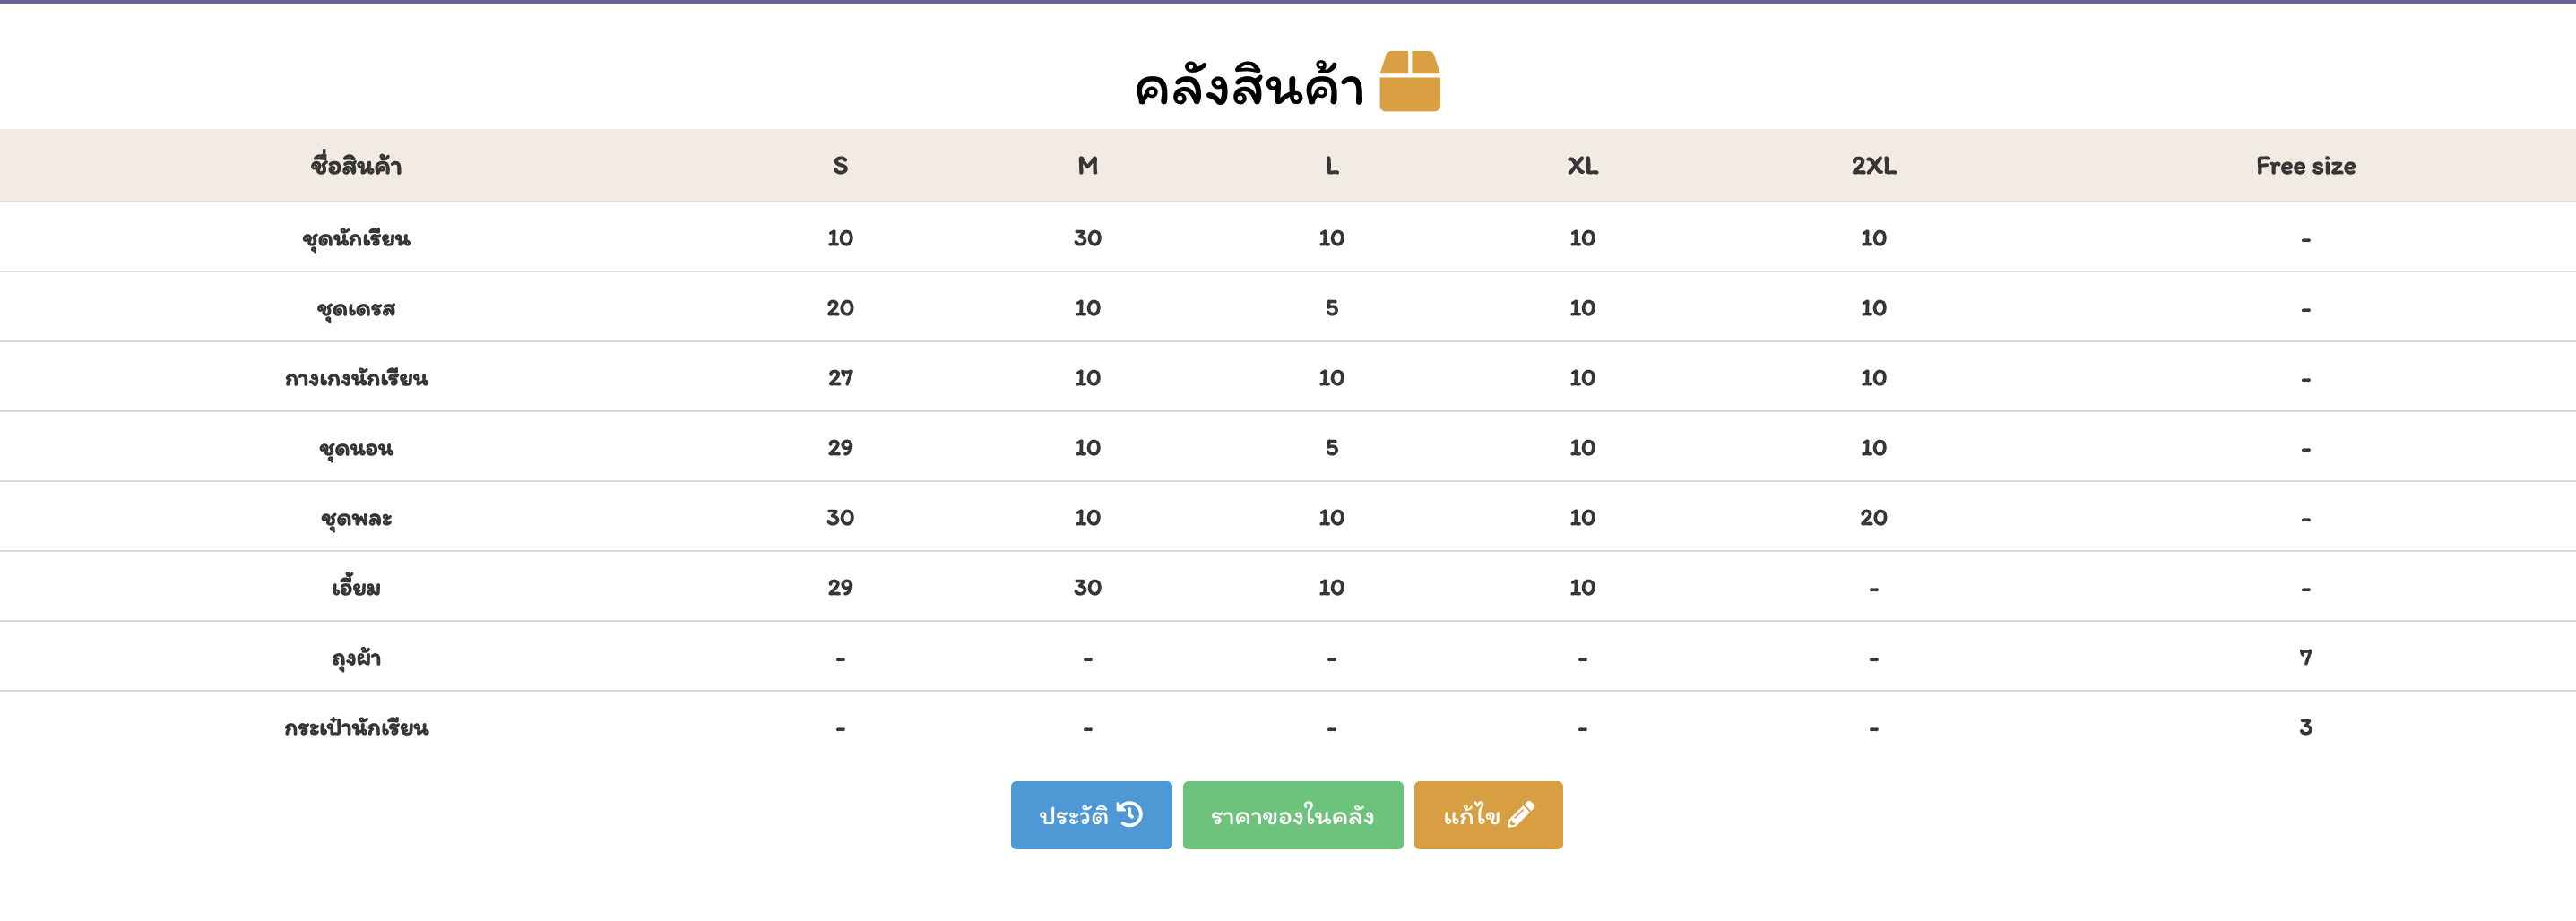
\includegraphics[width=\linewidth]{images/Stock.png}
  \end{center}
  \caption[Poem]{Stock Page}
  \label{fig:Stock}
  \end{figure}

\begin{figure}
  \begin{center}
  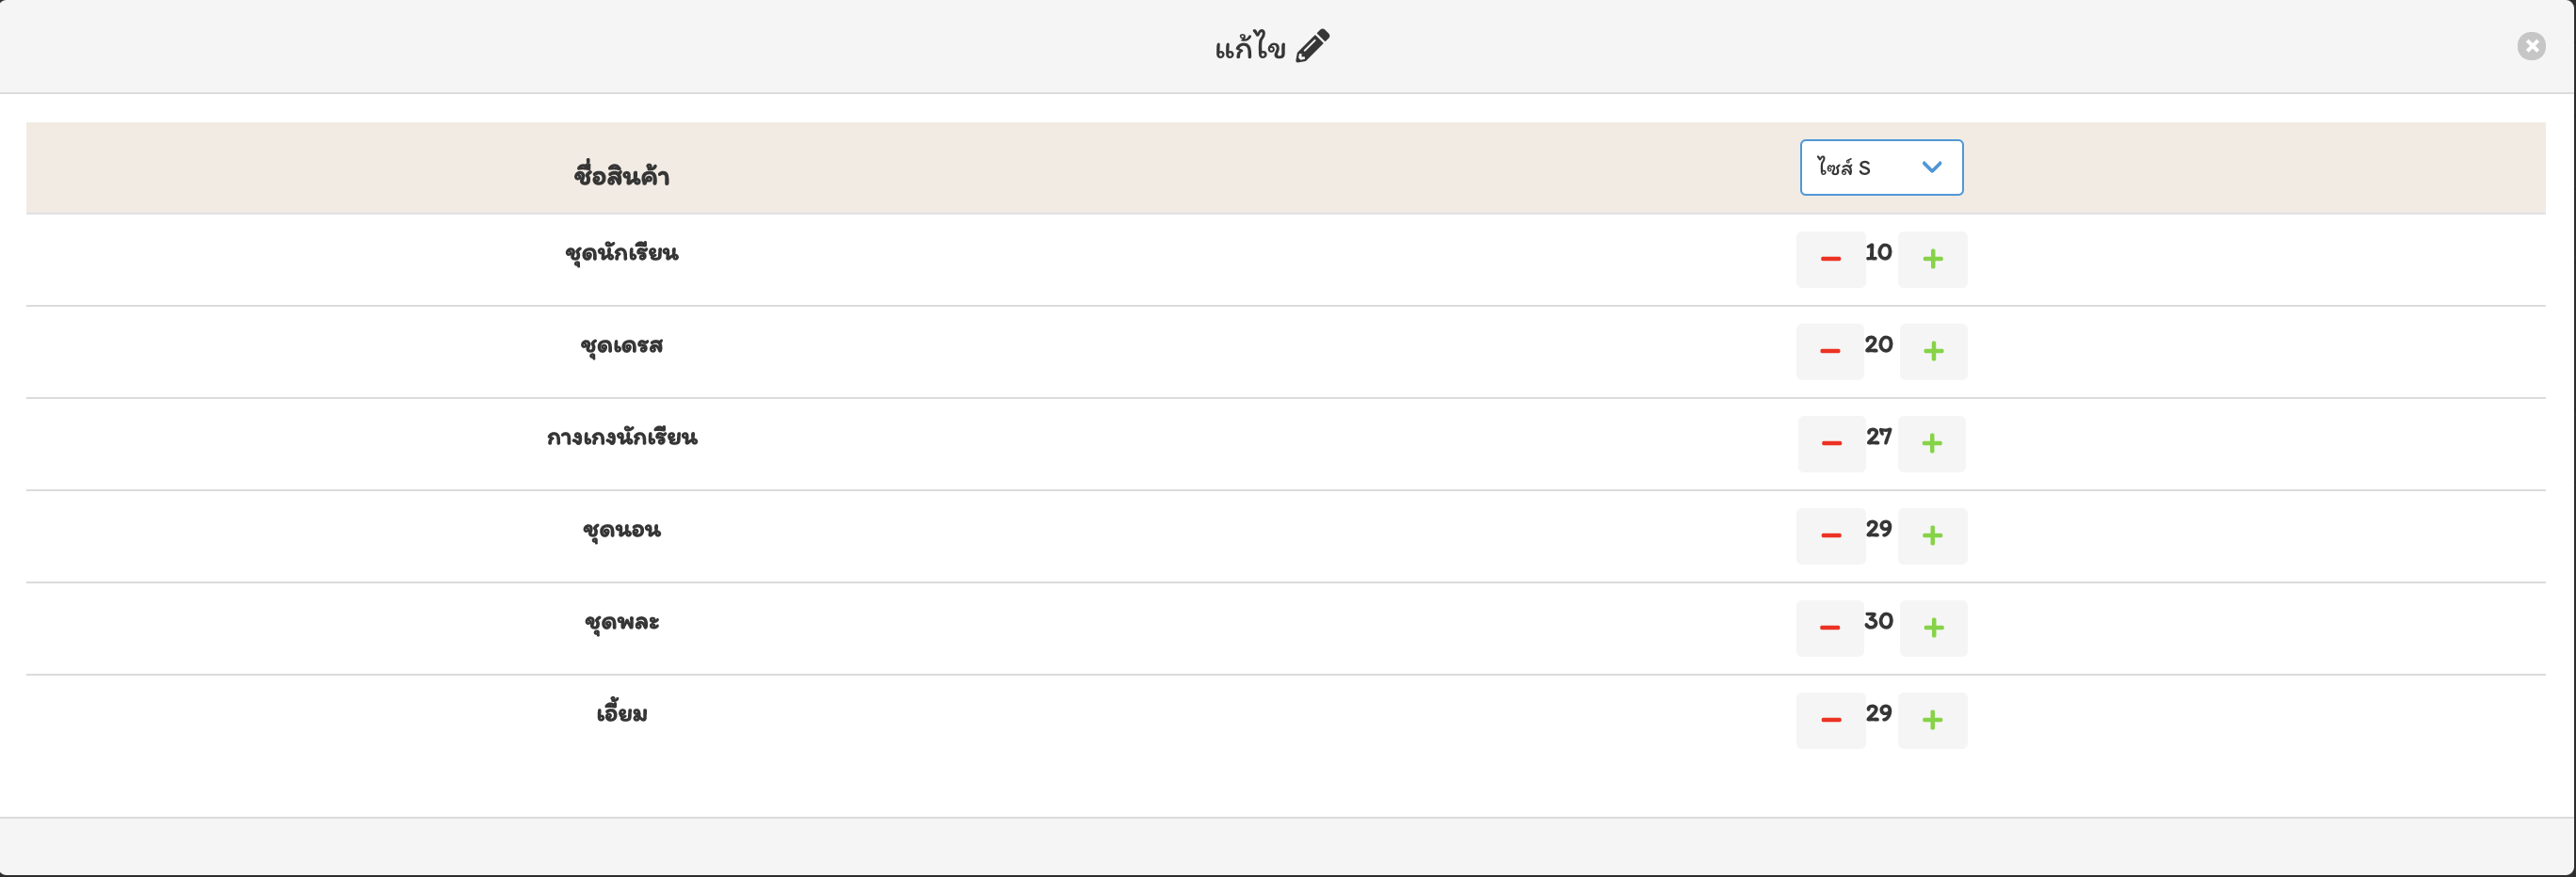
\includegraphics[width=\linewidth]{images/handleStock.png}
  \end{center}
  \caption[Poem]{Handle Stock Page}
  \label{fig:CheckStock}
  \end{figure}
\begin{figure}
  \begin{center}
  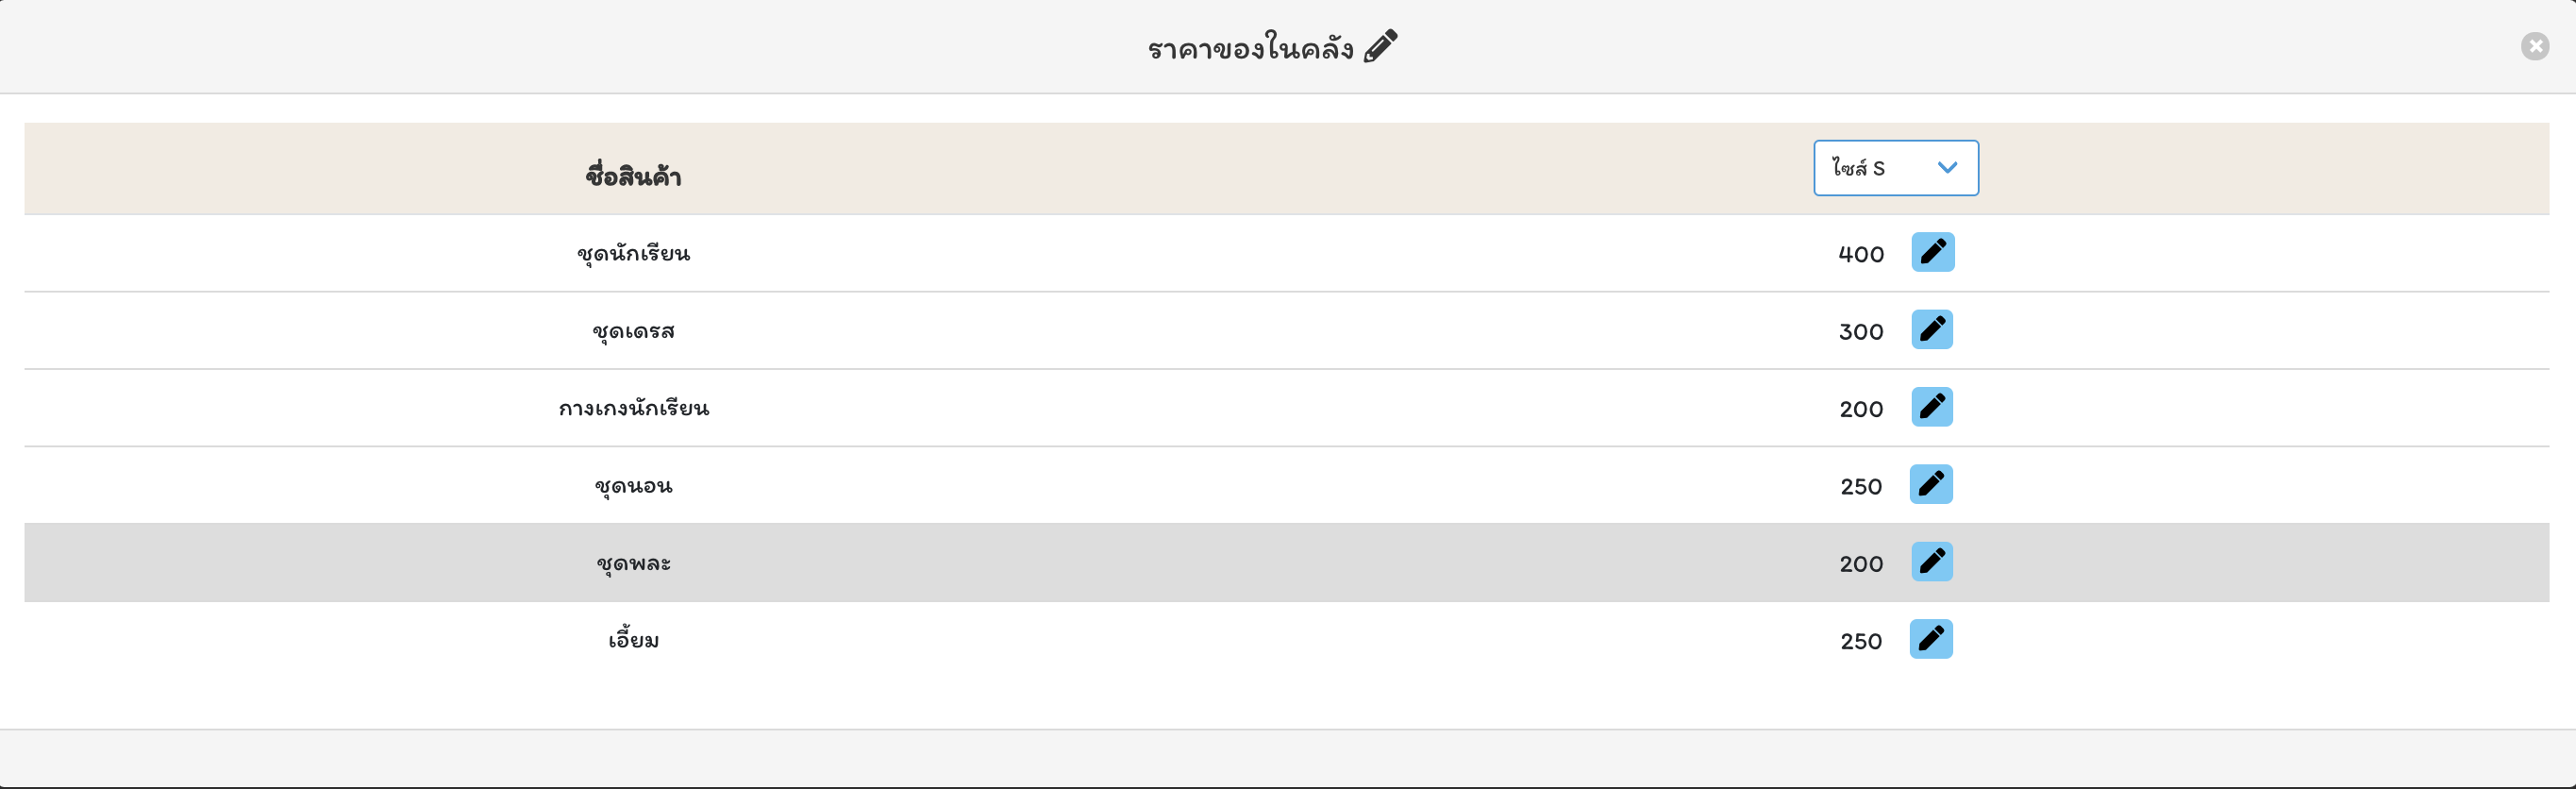
\includegraphics[width=\linewidth]{images/editPrice.png}
  \end{center}
  \caption[Poem]{Edit Stock Price Page}
  \label{fig:editPrice}
  \end{figure}
\begin{figure}
  \begin{center}
  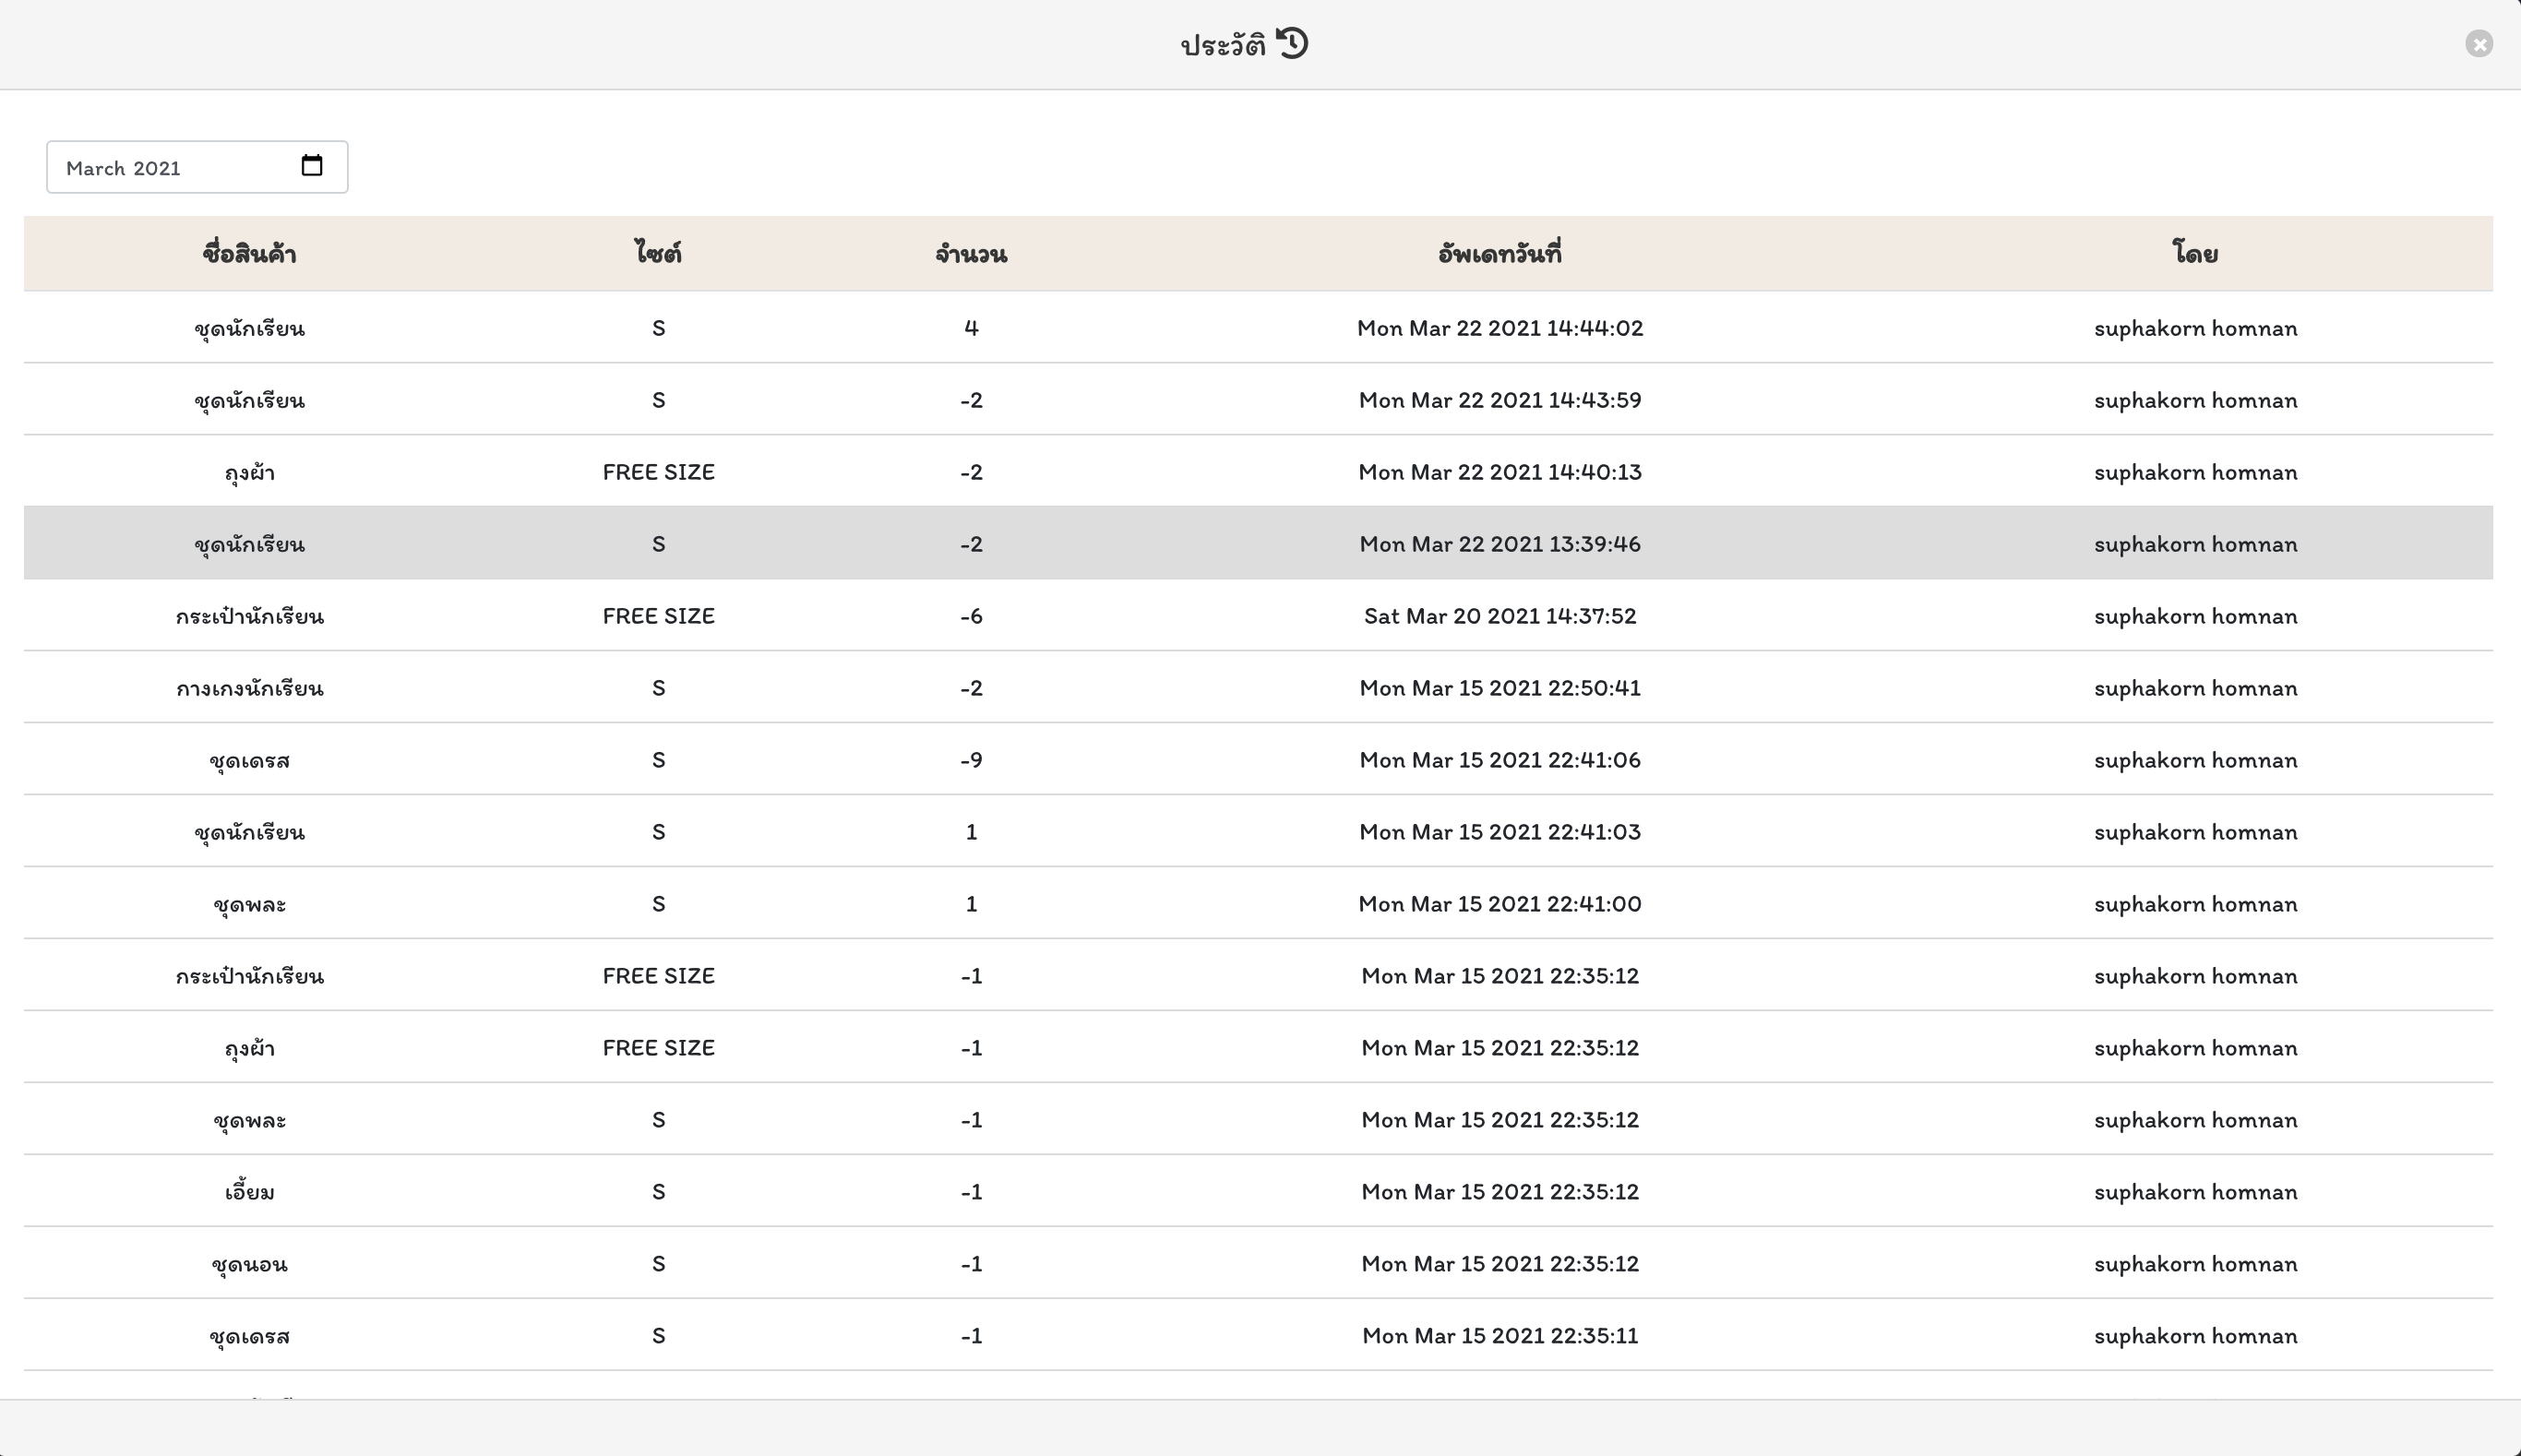
\includegraphics[width=\linewidth]{images/historyStock.png}
  \end{center}
  \caption[Poem]{Show History Stock Page}
  \label{fig:HistoryStock}
  \end{figure}
\begin{figure}
  \begin{center}
  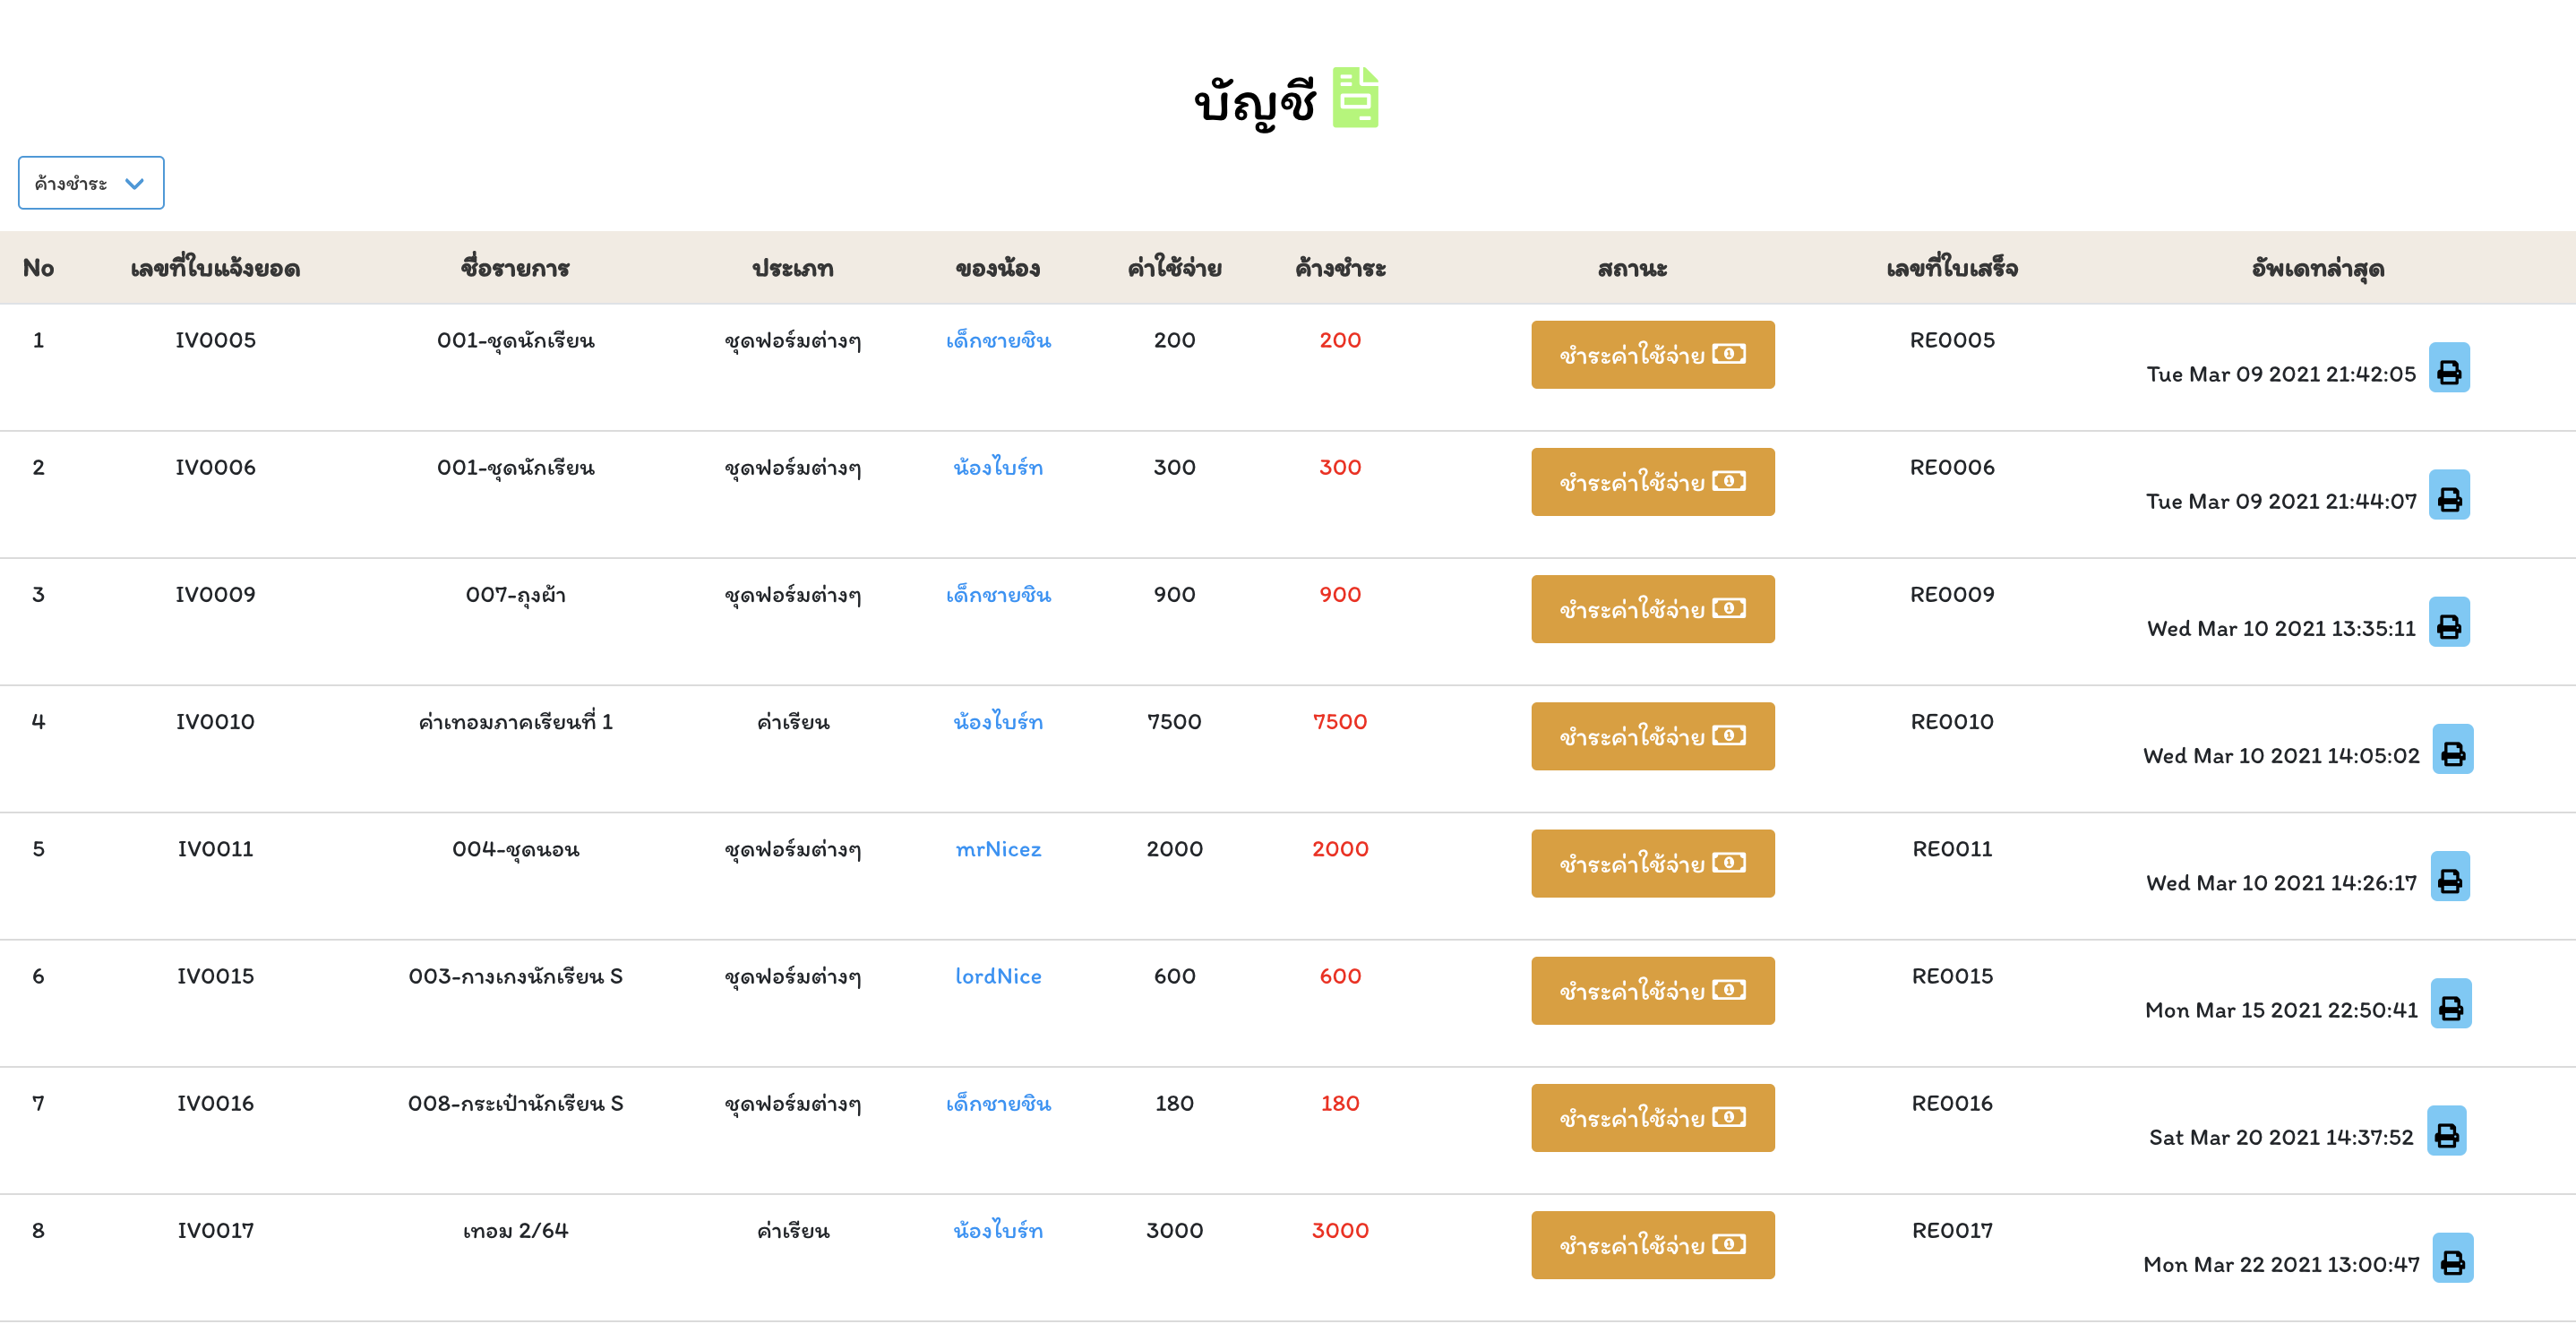
\includegraphics[width=\linewidth]{images/Payment.png}
  \end{center}
  \caption[Poem]{Payment Page}
  \label{fig:Payment}

  \end{figure}
\begin{figure}
  \begin{center}
  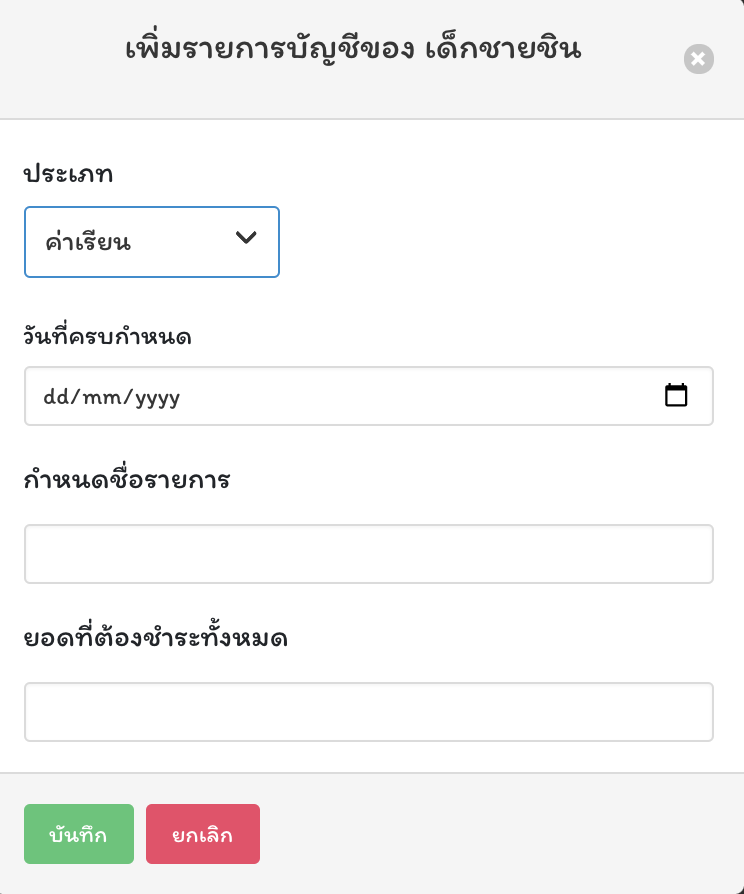
\includegraphics[width=\linewidth]{images/CreatePayment.png}
  \end{center}
  \caption[Poem]{CreatePayment}
  \label{fig:CreatePayment}
  \end{figure}
\begin{figure}
  \begin{center}
  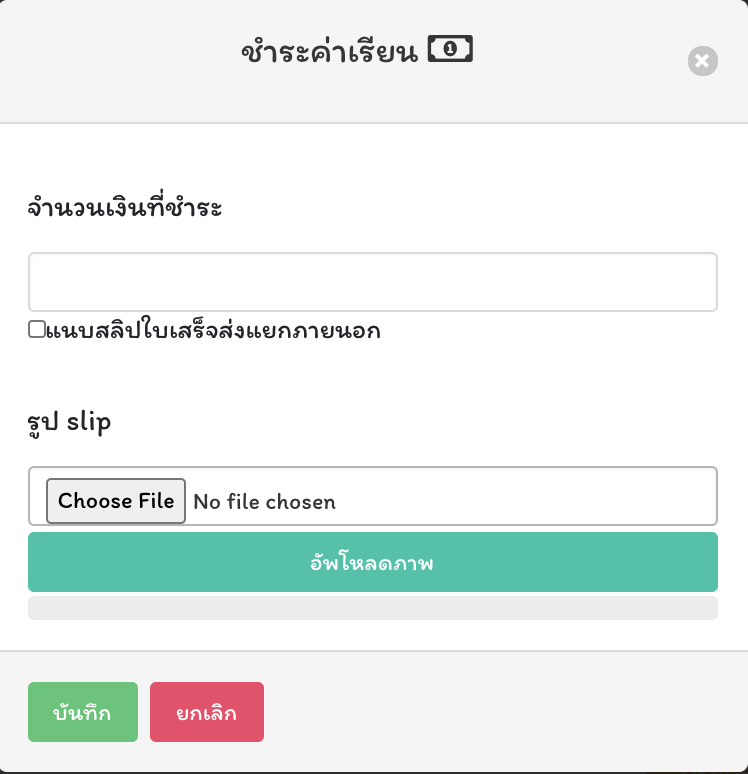
\includegraphics[width=\linewidth]{images/UpdatePayment.png}
  \end{center}
  \caption[Poem]{Handle Payment}
  \label{fig:updatePayment}
  \end{figure}
\begin{figure}
  \begin{center}
  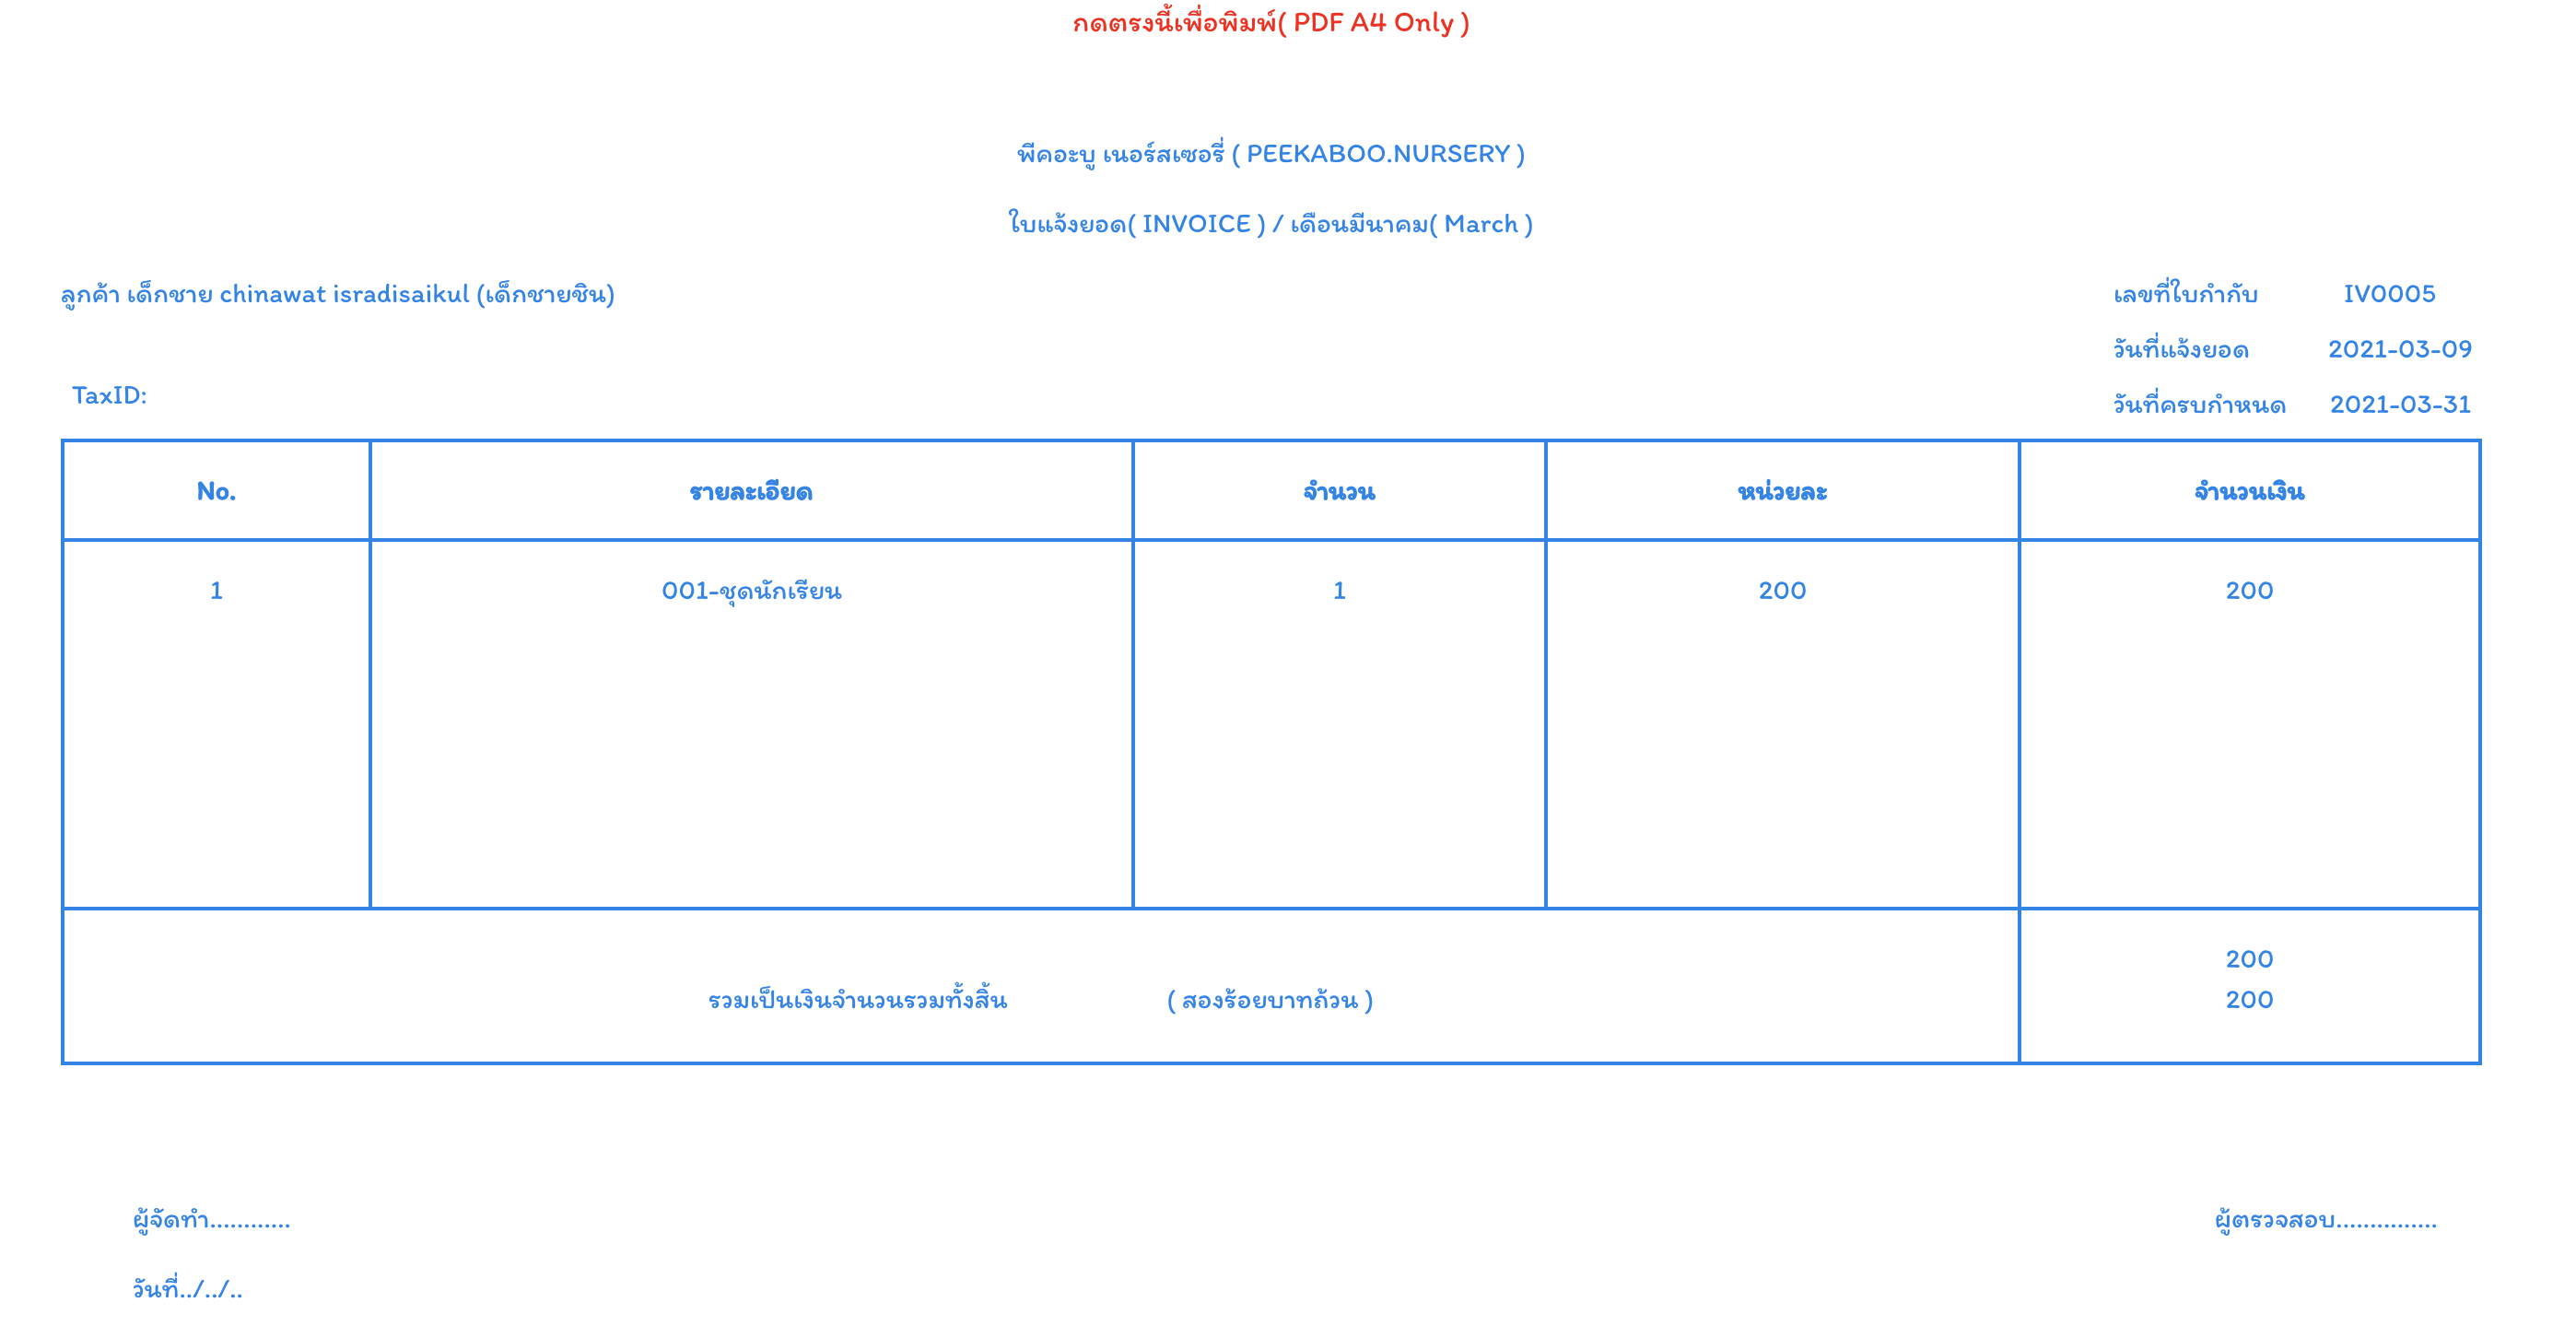
\includegraphics[width=\linewidth]{images/invoicePage.png}
  \end{center}
  \caption[Poem]{Page for printing invoice}
  \label{fig:invoicePage}
  \end{figure}
\begin{figure}
  \begin{center}
  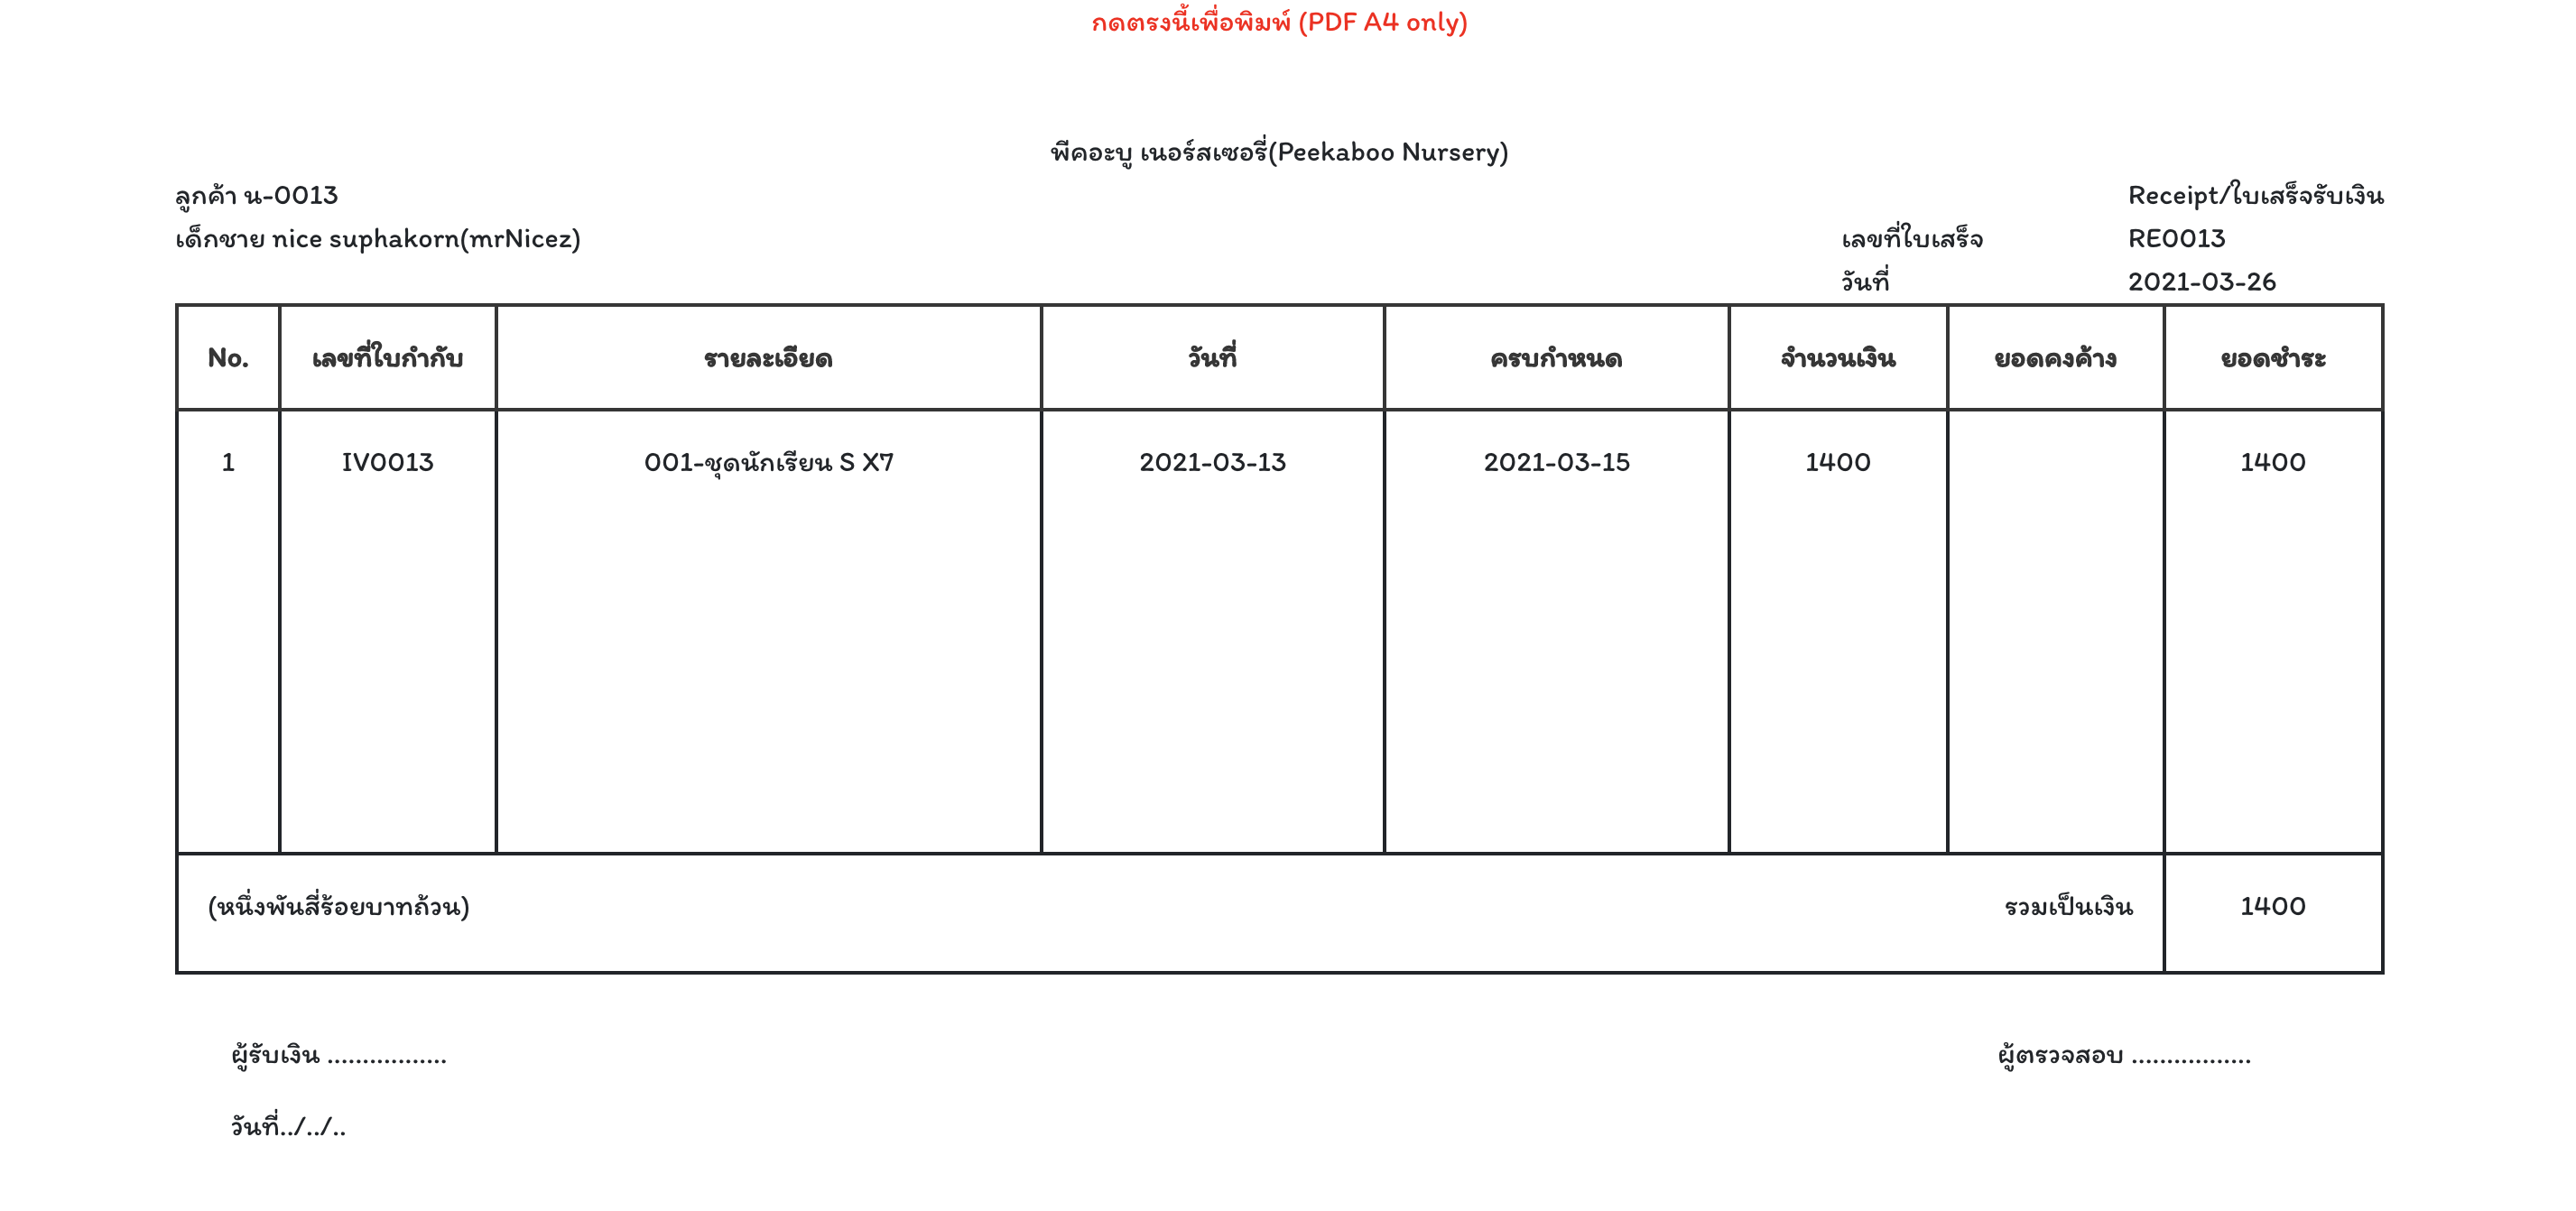
\includegraphics[width=\linewidth]{images/slipPage.png}
  \end{center}
  \caption[Poem]{Page for printing slip}
  \label{fig:slipPage}
  \end{figure}